%% POSIM - IPM Journal Submission
\documentclass[a4paper,fleqn]{cas-sc}

\usepackage[authoryear,longnamesfirst]{natbib}
\usepackage{amsmath}
\usepackage{algorithm}
\usepackage{algorithmic}
\usepackage{array}
\usepackage{graphicx}
\usepackage{booktabs}
\usepackage{multirow}
\usepackage{colortbl}
\usepackage{xcolor}
\usepackage{makecell}
\usepackage[most]{tcolorbox}
\usepackage{subfig}
\usepackage{wrapfig}
\usepackage{fontspec}
\setmainfont{Times New Roman}
\setsansfont{Arial}
\setmonofont{Courier New}
\ExplSyntaxOn
\cs_if_exist:cT { not= } { \cs_undefine:c { not= } }
\cs_if_exist:cT { not< } { \cs_undefine:c { not< } }
\cs_if_exist:cT { not> } { \cs_undefine:c { not> } }
\ExplSyntaxOff
\usepackage{unicode-math}
\setmathfont{XITS Math}

\usepackage{xeCJK}
\setCJKmainfont[BoldFont=SimHei,ItalicFont=KaiTi]{SimSun}
\setCJKsansfont{Microsoft YaHei}
\setCJKmonofont{FangSong}

\usepackage{listings}
\lstset{
  basicstyle=\scriptsize\ttfamily,
  breaklines=true,
  frame=none,
  columns=fullflexible,
  keepspaces=true,
  aboveskip=2pt,
  belowskip=2pt,
}
\usepackage{etoolbox}
\AtBeginEnvironment{tabular}{\fontspec{Times New Roman}}

\usepackage{caption}
\captionsetup{font={small,rm},labelfont={bf},labelsep=newline}
\captionsetup[table]{font={small,rm},labelfont={bf},labelsep=newline}
\captionsetup[figure]{font={small,rm},labelfont={bf},labelsep=newline}

\hypersetup{citecolor={blue!80!black},linkcolor={blue!80!black},urlcolor={blue!80!black}}
\graphicspath{{figures/}}

\definecolor{oursrow}{RGB}{232,245,233}
\definecolor{greenrow}{RGB}{228,245,228}
\definecolor{orangerow}{RGB}{232,245,233}
\definecolor{purplerow}{RGB}{232,245,233}
\definecolor{grayrow}{RGB}{240,250,240}
\definecolor{promptbg}{RGB}{242,247,253}
\definecolor{promptborder}{RGB}{70,130,180}
\definecolor{gaingreen}{RGB}{34,139,34}

\newtcolorbox{promptbox}{
 colback=promptbg, colframe=promptborder,
 boxrule=0.5pt, arc=1mm,
 left=4pt, right=4pt, top=4pt, bottom=4pt,
 breakable, enhanced}

\newcommand{\best}[1]{\textbf{#1}}
\newcommand{\na}{\text{---}}
\newcommand{\posim}{\textsc{Posim}}
\newcommand{\gain}[1]{{\scriptsize\textcolor{gaingreen}{\,#1}}}

\def\tsc#1{\csdef{#1}{\textsc{\lowercase{#1}}\xspace}}
\tsc{WGM}
\tsc{QE}

\begin{document}
\let\WriteBookmarks\relax
\def\floatpagepagefraction{1}
\def\textpagefraction{.001}

\shorttitle{POSIM：基于元认知智能体的社交媒体舆情仿真}
\shortauthors{作者等}

\title [mode = title]{POSIM：基于元认知智能体的通用社交媒体舆情仿真框架}

\author[1]{作者}[style=chinese]
\cormark[1]
\ead{}
\credit{Conceptualization, Methodology, Software, Writing - Original draft}

\affiliation[1]{organization={},
            city={},
            country={中国}}

\cortext[1]{通讯作者}

\begin{abstract}
社交媒体舆情事件可在数小时内引发大规模用户的参与讨论，理解并预判其演化过程对社会治理与危机应对具有重要价值。传统的舆情建模方法，如传染病模型和基于规则的代理模型（ABM），难以刻画真实社交用户的复杂认知过程，也缺乏环境感知和适应能力。本文提出通用社交媒体舆情仿真框架\textbf{POSIM}（\textbf{P}ublic \textbf{O}pinion \textbf{Sim}ulator），将大语言模型嵌入\textbf{融合情绪因素的BDI分层认知框架}，构建具有显式认知状态和可追溯决策链的元认知智能体。仿真环境基于\textbf{霍克斯自激点过程}统一建模外生事件冲击与内生用户交互，配合虚拟社交媒体平台的推荐与社交网络机制，支持分钟级时间分辨率下的长周期仿真，并通过高度解耦的模块化架构保证各核心组件的独立替换与功能扩展。验证层面，本文建立了\textbf{从微观行为机制到宏观涌现现象再到统计结果一致性的三层递进验证体系}。在从微博平台采集的多个舆情数据上的实验表明，POSIM生成的智能体行为在微观层面符合真实网民的认知机制，并成功涌现出舆情生命周期、情绪极化和无标度拓扑等与社会科学理论一致的宏观现象；在统计校准层面，模拟结果的行为、内容和拓扑指标相较于最优基线分别提升了\textbf{5.0\%}、\textbf{13.0\%}和\textbf{8.5\%}。进一步的案例研究表明，POSIM可作为计算实验平台支持多样的事前策略推演，为舆情治理提供可量化的决策依据。框架已开源于\url{https://github.com/DeepCog/POSIM}。
\end{abstract}

% \begin{highlights}
% \item 提出EBDI元认知智能体架构，将大语言模型嵌入分层认知框架实现具有可追溯决策链的舆情行为仿真
% \item 基于霍克斯自激点过程构建时间-事件混合驱动仿真环境，支持分钟级时间分辨率的长周期连续仿真
% \item 建立三层递进验证体系，在三个真实微博数据集上行为、内容和拓扑层面全面优于基线方法
% \item 高度解耦的模块化架构保证各组件独立替换与功能扩展，案例研究验证了框架在舆情治理场景中的应用价值
% \end{highlights}

\begin{keywords}
社交媒体仿真 \sep 舆情分析 \sep 大语言模型 \sep 智能体认知架构 \sep 霍克斯过程
\end{keywords}

\maketitle

% ============================================================
% 第1节 引言
% ============================================================
\section{引言}\label{sec:intro}

社交媒体已成为公共舆论形成与传播的核心场域，一则突发事件可在数小时内引发大规模用户的参与讨论，形成复杂的群体情绪动态~\citep{gonzalez_emotional_2010}和信息级联~\citep{goldstein_structure_2012}。理解和预判舆情演化规律对社会治理、危机应对和公共政策制定具有重要的现实意义。然而，真实世界的社会实验面临伦理约束、不可重复性和变量不可控等根本性困难，使得基于计算机仿真的实验方法成为兼具科学严谨性和实践可操作性的研究路径~\citep{bonabeau_agent-based_2002}。

尽管如此，构建与真实舆情过程在微观机制和统计结果上均高度一致的仿真系统仍面临个体认知建模粗糙、时间动力学精度有限以及验证体系单一等多重挑战~\citep{kramer_experimental_2014,zhao_seismic_2015,mcculloch_calibrating_2022}。传统的舆情传播建模方法，如传染病模型~\citep{daley_stochastic_1965}和阈值级联模型~\citep{granovetter_threshold_1978}，将个体抽象为离散状态节点，虽能揭示宏观扩散规律，但对个体异质性、语义内容与互动策略的表达能力有限。与上述宏观扩散模型不同，基于智能体的建模（ABM）方法作为一种通用范式，因其自下而上的涌现特性在计算仿真中获得了广泛关注~\citep{macal_tutorial_2010}，因此有大量研究将观点动力学模型作为 ABM 的关键组成，通过预设的意见表示与更新规则刻画社会影响下的观点演化~\citep{castellano_statistical_2009}。ABM方法是舆情仿真的重要路径，但规则驱动的智能体仍无法产生接近真实的社交互动，仿真停留在数值层面，固定规则也难以覆盖网民认知决策的复杂性与非理性特征。

\begin{table}[!t]
\centering
\caption{Comparison of POSIM with existing public opinion simulation platforms. ``$\bigstar$'' count indicates capability level (1--5). $\checkmark$ = supported, $\times$ = unsupported.}
\label{tab:comparison}
\footnotesize
\renewcommand{\arraystretch}{1.0}
\begin{tabular}{@{}lcccccc@{}}
\toprule
\textbf{Platform} & \makecell{\textbf{Cognitive}\\\textbf{Mechanism}} & \makecell{\textbf{Real-Data}\\\textbf{Validation}} & \makecell{\textbf{Strategy}\\\textbf{Evaluation}} & \makecell{\textbf{Multi-Type}\\\textbf{Agents}} & \makecell{\textbf{Temporal}\\\textbf{Precision}} & \makecell{\textbf{Scala-}\\\textbf{bility}} \\
\midrule
S3~\citep{gao_s3_2023} & $\times$ & $\checkmark$ & $\times$ & $\times$ & $\bigstar\bigstar\bigstar$ & $\bigstar\bigstar\bigstar$ \\
HiSim~\citep{mou_unveiling_2024} & $\times$ & $\checkmark$ & $\times$ & $\checkmark$ & $\bigstar\bigstar$ & $\bigstar\bigstar$ \\
GA-S3~\citep{liu_agent-based_2024} & $\times$ & $\checkmark$ & $\times$ & $\checkmark$ & $\bigstar\bigstar\bigstar$ & $\bigstar\bigstar$ \\
SPARK~\citep{zhang_spark_2025} & $\times$ & $\times$ & $\times$ & $\checkmark$ & $\bigstar\bigstar$ & $\bigstar\bigstar$ \\
FDE-LLM~\citep{yao_social_2025} & $\times$ & $\checkmark$ & $\times$ & $\checkmark$ & $\bigstar\bigstar$ & $\bigstar\bigstar$ \\
TrendSim~\citep{zhang_trendsim_2025} & $\times$ & $\times$ & $\times$ & $\checkmark$ & $\bigstar\bigstar\bigstar\bigstar$ & $\bigstar\bigstar\bigstar$ \\
OASIS~\citep{yang_oasis_2025} & $\times$ & $\times$ & $\times$ & $\times$ & $\bigstar\bigstar\bigstar\bigstar$ & $\bigstar\bigstar\bigstar\bigstar$ \\
LMAgent~\citep{liu_lmagent_2026} & $\times$ & $\checkmark$ & $\times$ & $\checkmark$ & $\bigstar\bigstar$ & $\bigstar\bigstar$ \\
\midrule
\rowcolor{oursrow}
\textit{\textbf{POSIM (Ours)}} & $\checkmark$ & $\checkmark$ & $\checkmark$ & $\checkmark$ & $\bigstar\bigstar\bigstar\bigstar\bigstar$ & $\bigstar\bigstar\bigstar\bigstar\bigstar$ \\
\bottomrule
\end{tabular}
\end{table}

近年来，大语言模型（LLM）的突破为社会仿真注入了新的可能性~\citep{wang_survey_2024}。以生成式智能体~\citep{park_generative_2023}为代表的研究证明了LLM驱动的智能体具备涌现复杂社会行为的潜力，后续工作进一步将其应用于舆情仿真~\citep{gao_s3_2023,chuang_simulating_2024}，使智能体能够生成真实的文本内容并展现丰富的交互行为，并且具有极强的环境适应能力。然而，多数现有工作将LLM作为端到端的行为映射器，直接从环境输入映射到行为输出，缺乏显式的中间认知状态建模，长周期仿真中智能体的行为机制也难以保证。

为应对上述挑战，本文提出社交媒体舆情仿真框架POSIM（\textbf{P}ublic \textbf{O}pinion \textbf{Sim}ulator）。该框架的核心思想是将LLM作为决策引擎嵌入融合情绪因素的BDI（Belief-Desire-Intention）分层认知架构~\citep{bratman_intention_1987,rao_bdi_1995}，构建具备显式认知状态和可追溯决策链的元认知智能体。在仿真环境层面，基于霍克斯自激点过程~\citep{hawkes_spectra_1971}建模群体活跃强度的时间动力学，并构建包含推荐算法和社交网络的虚拟社交媒体平台，支持分钟级时间分辨率下的长周期连续仿真。在验证层面，建立从微观行为机制校准到宏观涌现现象校准再到统计结果一致性校准的三层递进验证方法论~\citep{sargent_verification_2013}。本文的主要贡献概括如下：

\begin{itemize}
\item 提出融合情绪因素的BDI元认知智能体架构（EBDI），将LLM嵌入分层认知框架，构建从感知到行为的完整认知链路，实现认知状态的显式建模与可追溯的决策生成。
\item 设计时间-事件混合驱动仿真环境，基于霍克斯自激点过程统一建模外生事件与内生交互的时间动力学，同时采用高度解耦的模块化架构来支持多场景仿真的灵活扩展。
\item 建立从微观行为机制到宏观涌现现象再到统计结果一致性的三层递进验证体系，在多个大规模真实微博舆情数据集上系统验证了框架的仿真一致性，并通过案例研究展示了框架在舆情治理场景中的应用价值。
\end{itemize}

% ============================================================
% 第2节 相关工作
% ============================================================
\section{相关工作}\label{sec:related}

\subsection{舆情传播建模}

舆情传播建模旨在刻画公众信息在社会网络中扩散与演化的动力学机制。早期研究往往沿用传染病学展开，例如随机谣言传播模型~\citep{daley_stochastic_1965}将个体划分为无知者、传播者和免疫者三类状态。后续工作引入复杂网络拓扑~\citep{watts_strogatz_1998,barabasi_albert_1999}和多阶段转移机制~\citep{jiang_weibo_spnr_2020}以分析网络结构对级联规模的影响，而阈值级联模型~\citep{granovetter_threshold_1978,watts_cascades_2002}则从个体决策阈值角度解释群体行为的涌现。除了网络科学的视角，系统动力学~\citep{forrester_industrial_1961,sterman_business_2000}通过存量流量图和反馈环路对传播主体之间的因果关系进行建模~\citep{gao_sd_public_opinion_2019,liu_evolution_2024}，能够从宏观刻画系统变量对舆情走向的影响，但其局限在于将群体视为连续的宏观流量而非具有个性化特征的异质个体。在时间动力学分析方面，自激点过程~\citep{hawkes_spectra_1971}为社交媒体级联现象提供了连续时间的参数化手段，SEISMIC~\citep{zhao_seismic_2015}和HIP~\citep{rizoiu_expecting_2017}等模型分别从自激机制和内外生统一的角度预测了内容的流行度，近期的工作则进一步将观点极性融入多变量标记霍克斯过程~\citep{zhang_opinion-aware_2023}，但依然不可避免地将个体的复杂心理过程折叠进了少量的数学参数中。总体而言，上述方法在预测群体趋势方面各有所长，却均难以深入到个体认知过程的显式建模，这种自上而下抽象方式的局限促使研究者逐渐转向基于智能体的建模范式。

\subsection{基于智能体的建模与观点动力学}

基于智能体的建模（ABM）通过赋予大量异质个体局部行为规则并观察群体涌现，成为社会系统自下而上研究的核心范式~\citep{bonabeau_agent-based_2002,macal_tutorial_2010}，ODD协议~\citep{grimm_odd_2010}和参数标定方法~\citep{mcculloch_calibrating_2022}进一步为其提供了可复现建模与系统性验证的规范化流程。该范式在观点动力学领域取得了丰硕成果，DeGroot共识模型~\citep{degroot_reaching_1974}通过加权平均描述观点趋同，Deffuant-Weisbuch模型~\citep{deffuant_mixing_2000}引入成对交互刻画局部说服，Hegselmann-Krause有界置信模型~\citep{hegselmann_opinion_2002}则借助选择性暴露解释群体分裂，这一系列工作系统性地复现了从共识到极化的相变现象~\citep{castellano_statistical_2009,bernardo_bc_survey_2024}。在此基础上，研究者进一步在社交网络上构建了包含多类智能体的舆情仿真系统~\citep{chen_evolution_2025,wu_public_2023}，用以探究极化与回音室效应的形成机理~\citep{liu_agent-based_2024,banisch_agent_2012,cinelli2021echo_ipm}。然而，ABM方法的智能体的决策逻辑完全依赖于预定义的数值规则，观点被简化为低维连续变量，交互被约束为加权平均或阈值函数。这种规则驱动的范式既无法感知真实舆情场中纷繁复杂的外部环境信息，也无法模拟社交网民认知中涉及的情感演化、动机推理和自主决策等高级过程。

\subsection{大语言模型驱动的社会仿真}

人工智能正在经历从感知智能向认知智能的深刻过渡，大语言模型所具备的语义理解、上下文推理和自主决策能力，为社会仿真带来了超越传统规则范式的全新可能~\citep{wang_survey_2024}。生成式智能体~\citep{park_generative_2023}率先展示了大模型在自主规划与社会互动中的涌现能力，随后面向社交媒体的仿真研究迅速展开（如表~\ref{tab:comparison}所示）。S3~\citep{gao_s3_2023}较早地搭建了基于大模型的信息传播仿真框架，验证了语言模型驱动智能体进行社交互动的可行性。在此基础上，SPARK~\citep{zhang_spark_2025}和LLM-AIDSim~\citep{zhang_llm-aidsim_2025,hu_llm-enhanced_2024}进一步探索了立场演化与信息扩散的涌现规律，FDE-LLM~\citep{yao_social_2025}则创新性地将动力学方程与语言模型融合，为观点轨迹提供了数学层面的约束。在仿真规模与效率方面，OASIS~\citep{yang_oasis_2025}将节点规模显著提升至百万级，展现了大模型驱动仿真的可扩展潜力；HiSim~\citep{mou_unveiling_2024}则采用混合驱动策略，在计算效率与模拟保真度之间取得了较好的平衡；TrendSim~\citep{zhang_trendsim_2025}进一步尝试模拟了热搜话题的演化过程。上述工作取得了重要进展，但其普遍将大模型作为端到端的行为决策器，缺乏对用户复杂认知链路的显式建模；同时，这些工作主要聚焦于社交网络中的观点传播，而真实舆情事件具有独特的社会心理背景、多元的参与群体和复杂的演化模式，现有框架尚难以充分刻画这种复杂性；此外，多数平台在验证层面缺乏基于仿真学理论的系统性校验，难以从机制层和结果层校准模拟与真实舆情之间的一致有效性。

针对这些局限，本文提出的POSIM框架通过EBDI分层认知架构赋予每个智能体显式且个性化的认知决策链路，在高精度霍克斯点过程时间引擎驱动和虚拟社交媒体平台下构建了贴近真实舆情发生的仿真环境，并建立了覆盖微观行为机制校准、宏观涌现校验和统计结果一致性校准的三层递进验证体系，同时框架的模块化设计保证了向多种应用场景扩展的能力。

% ============================================================
% 研究目标（IPM要求）
% ============================================================
\section{研究目标}\label{sec:objective}

“\textit{All models are wrong, but some are useful}。”~\citep{box_draper_1987_emprical_modelbuilding}舆情仿真研究的关键不在于追求对现实的逐点复刻，而在于在可解释、可验证的前提下，获得对舆情机制与演化规律\textbf{足够可信且可用于决策}的近似。传统ABM方法具备自下而上的涌现优势却缺乏认知深度与语义生成能力。大语言模型展现出强大的信息处理与语义推理能力，使得在仿真中以自然语言为载体统一表示用户决策过程成为可能，从而为构建更接近真实用户认知机制的决策模型提供了新的技术基础。受此启发，本研究将大语言模型与结构化认知架构相融合，构建一个兼具认知保真度、时间动力学精度与验证完备性的通用舆情仿真框架，使仿真智能体不仅能够生成接近真实的社交行为与文本内容，还能够在尽量少的显式规则下涌现出与社会科学理论一致的群体现象。

形式化地，社交媒体舆情仿真的目标定义如下：给定一组初始用户群体$\mathcal{U}$、事件背景$\mathcal{B}$及外部事件序列$\mathcal{E} = \{e_1, e_2, \ldots, e_K\}$，在虚拟社交媒体平台上模拟用户群体在舆情事件中的行为演化过程$\{A_t\}_{t=0}^{T}$，使得仿真产生的宏观统计特征与真实舆情数据具有统计一致性，同时智能体的微观决策过程具备认知可解释性。

具体而言，POSIM为每个由大语言模型驱动的智能体维护显式的信念（Belief）、欲望（Desire）与意图（Intention）等认知状态，并在分层BDI认知架构中引入情绪调制机制，使智能体能够在“感知—理解—评估—规划—行动”的链路上进行类人决策。在环境层面，POSIM采用霍克斯自激点过程作为统一的时间引擎，以刻画舆情过程中由外生事件冲击与内生交互反馈共同驱动的非平稳活跃强度，进而支持分钟级时间分辨率下的长周期连续仿真。在可信度评估层面，POSIM进一步建立从微观行为机制校准、到宏观涌现现象检验、再到统计结果一致性对齐的三层递进验证体系，系统性地确立仿真输出在机制、现象与数据三个层面的可靠性。最后，得益于高度解耦的模块化设计，框架各核心组件可通过标准接口独立替换与扩展，从而能够自然地支持社会科学实验以及治理策略研究等更广泛的应用场景。

% ============================================================
% POSIM框架
% ============================================================
\section{POSIM框架}\label{sec:method}

本节详细介绍POSIM框架的三个核心组件，分别为元认知智能体架构（第\ref{subsec:agent}节）、仿真环境（第\ref{subsec:env}节）和策略推演（第\ref{subsec:strategy}节）。图~\ref{fig:framework}展示了框架的整体架构。

\begin{figure}[!t]
\centering
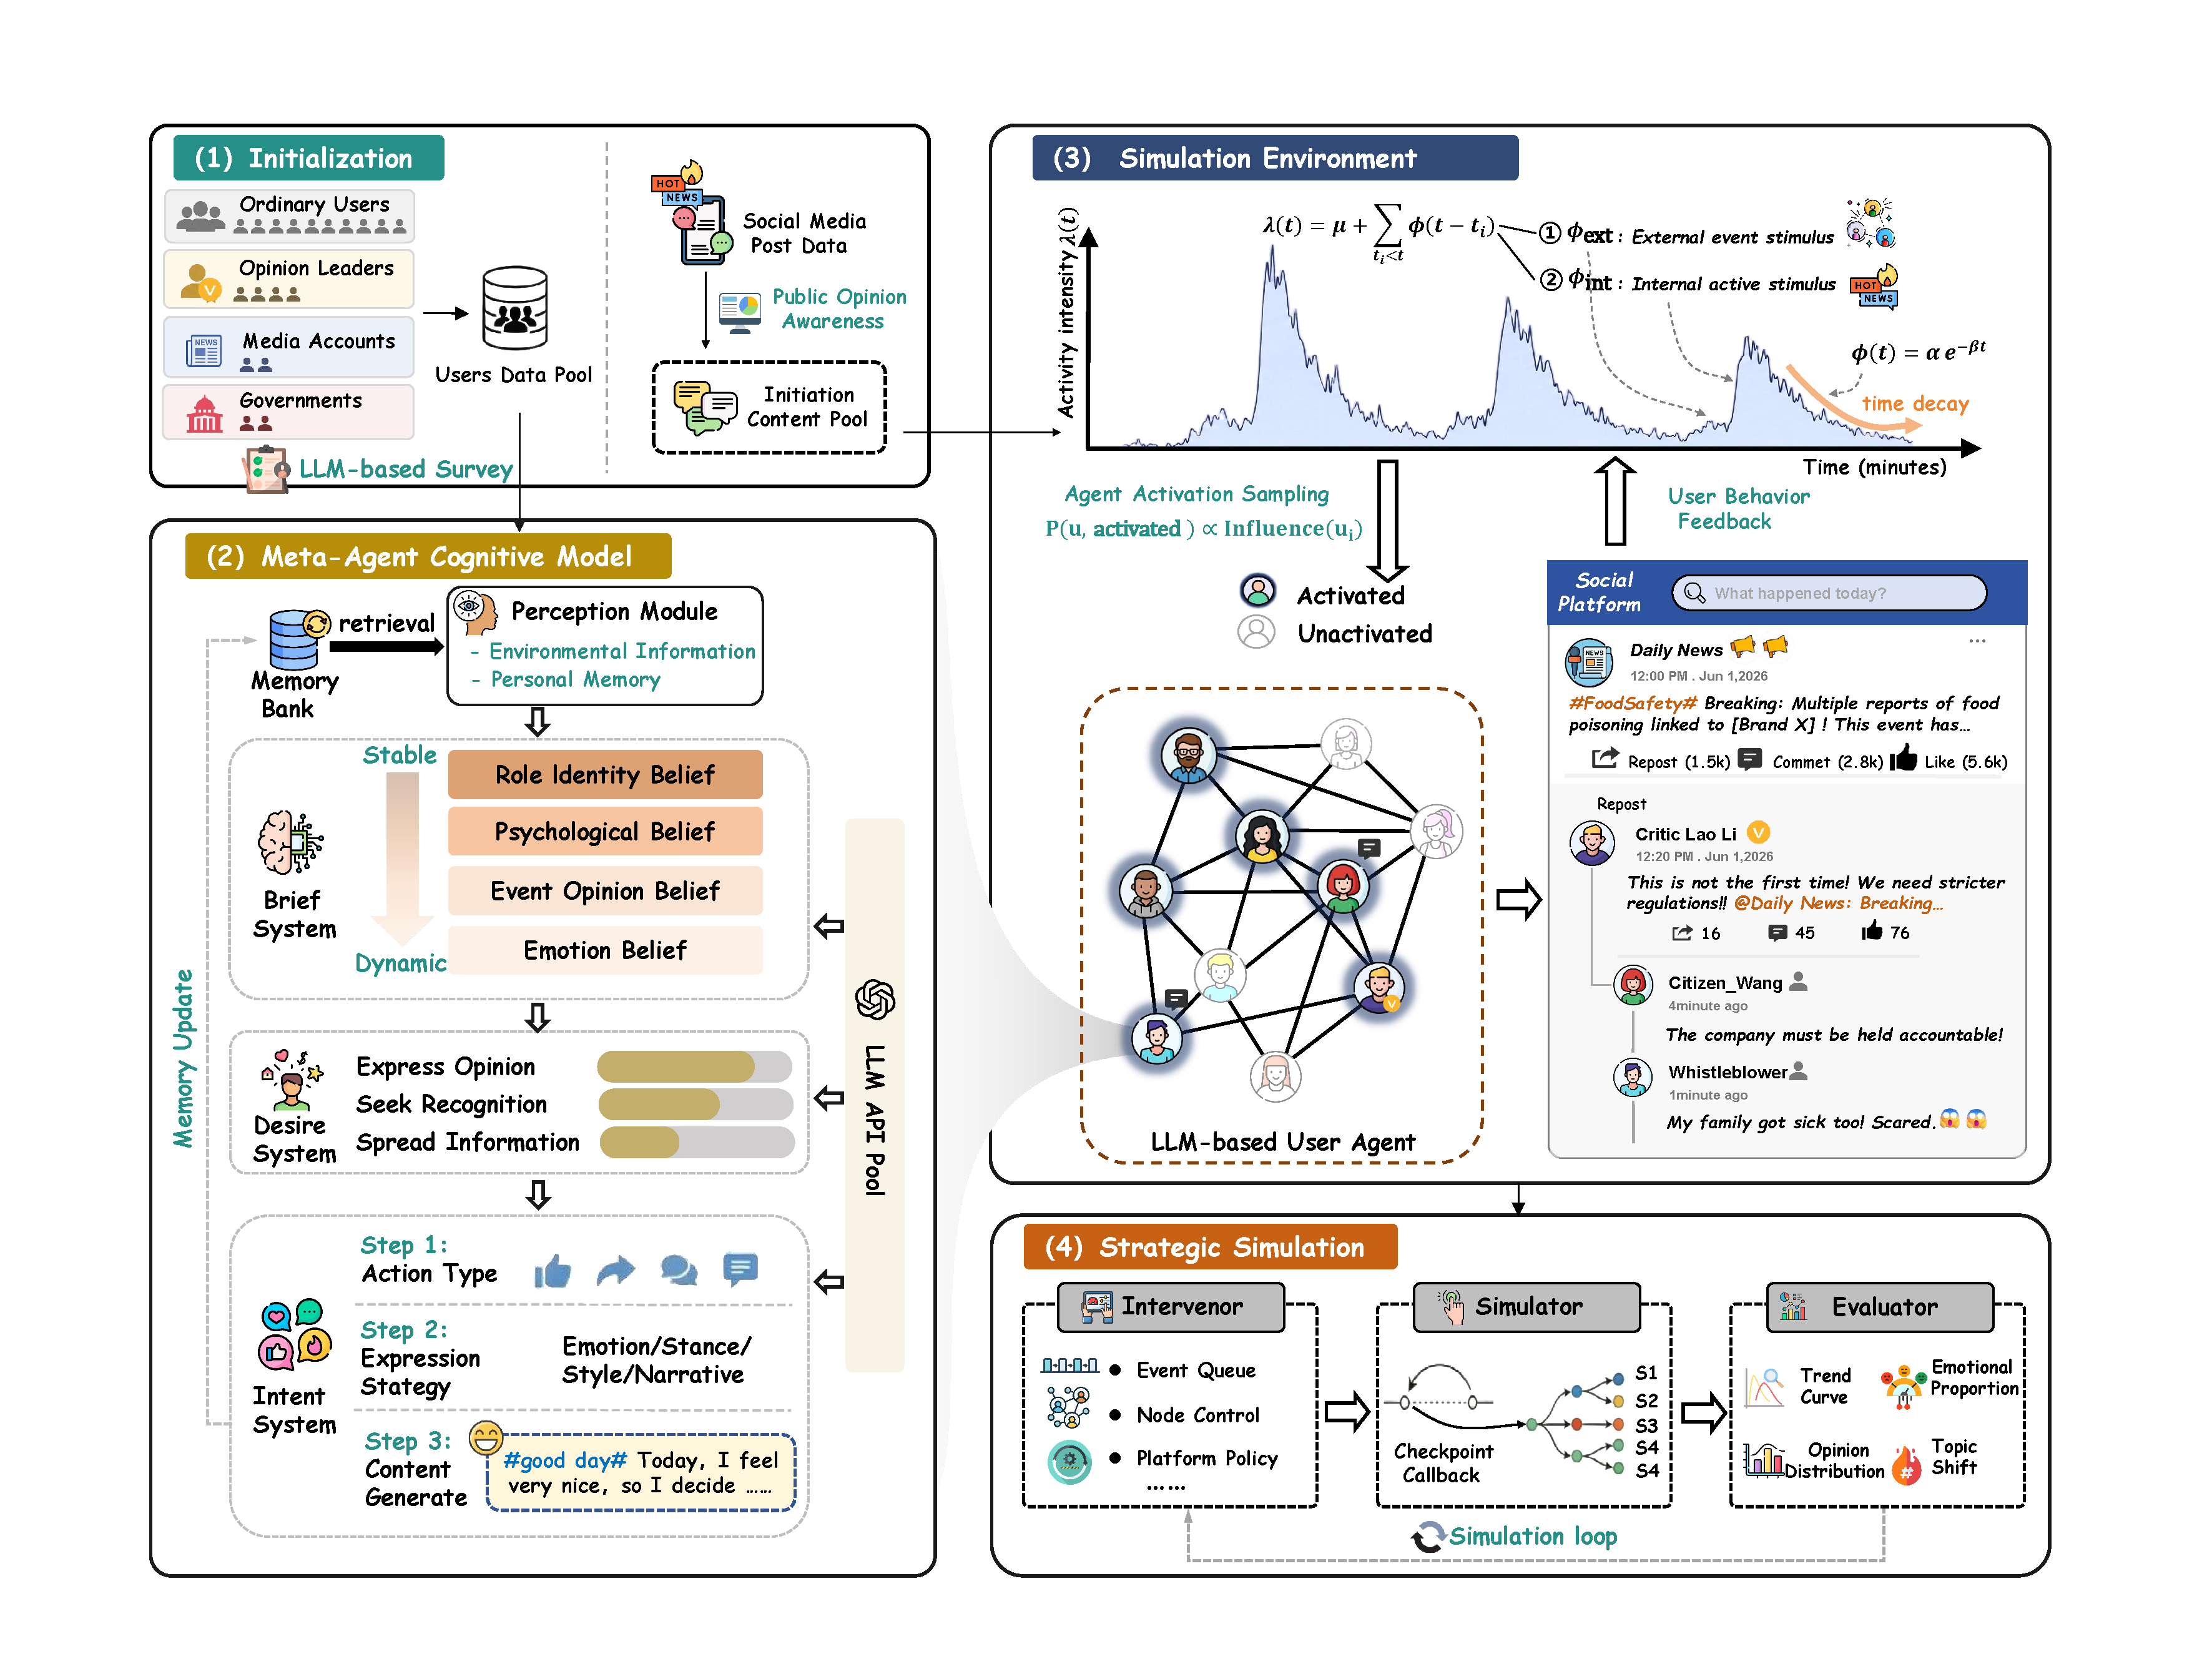
\includegraphics[width=0.92\textwidth]{framework_overview.pdf}
\caption{POSIM框架总体架构。(1)~初始化模块基于真实用户数据和LLM驱动的深度访谈生成多类型智能体（普通用户、意见领袖、媒体账号、政府账号）的初始认知状态；(2)~元认知智能体架构（左侧）实现感知$\to$信念$\to$欲望$\to$意图$\to$行为的EBDI认知决策链路，信念系统包含角色身份、心理认知、事件观点和情绪四类信念，意图系统通过三阶段推理生成行为类型、表达策略和具体内容；(3)~仿真环境（中上）由霍克斯自激点过程驱动的时间引擎控制智能体激活，虚拟社交媒体平台提供个性化推荐和社交网络交互；(4)~策略推演（右下）由干预器、仿真器和评估器三个模块组成，支持事件队列注入、节点控制和平台策略等多种干预手段，仿真器通过检查点回调机制生成多条平行演化轨迹以支持反事实推理，评估器从热度曲线、情感比例、观点分布和话题迁移等维度量化干预效果。}
\label{fig:framework}
\end{figure}

\subsection{元认知智能体架构}\label{subsec:agent}

传统的反应式智能体遵循简单的感知到行动模式，仅作为无状态的行为生成器，无法捕捉社交用户决策中涉及的复杂认知机制。考虑到社交媒体用户的行为决策受情绪驱动、认知偏差和社交影响等多重非理性因素的交互作用，且情绪与意图的深度耦合是危机事件演化的核心动力~\citep{myint2024crisis_mtl_intent}，我们在经典BDI（信念-欲望-意图）认知架构~\citep{bratman_intention_1987,rao_bdi_1995}的基础上，融入情感维度，提出EBDI元认知智能体架构。元认知主要体现在两个层面：智能体具有显式的自我认知状态，每一步决策均基于可观测的认知状态变化；智能体的认知过程本身是可审计的多阶段决策链~\citep{wei_chain_2022}，而非单次黑箱调用。认知流程形式化为：
\begin{equation}
\text{Perception}(P_t) \!\to\! \text{Belief}(B_t) \!\to\! \text{Desire}(D_t) \!\to\! \text{Intention}(I_t) \!\to\! \text{Action}(A_t)
\end{equation}

该架构以LLM为认知推理引擎，包含信念子系统、欲望子系统和意图子系统三个核心模块。三个子系统在每个决策周期内依次运行，各自接收上游输出作为输入，形成从环境感知到行为输出的完整且可追溯的认知链路。

\subsubsection{信念子系统}

信念是智能体对外部世界和自身状态的动态认知表征，构成一切决策推理的基础。社会心理学研究表明，个体的不同认知层次具有不同的稳定性，核心人格特质在短期内高度稳定，而对特定事件的观点和即时情绪则随信息输入快速变化。基于这一认知分层特性，并结合真实社交媒体网民的实际特点，我们设计了层次化的信念体系$B = \langle B^{id}, B^{psy}, B^{evt}, B^{emo} \rangle$，四类信念按认知修正难度从高到低排列。

\textbf{角色身份信念}$B^{id}$表征智能体的固有基础认知，包括人口学属性（性别、地域）、社交属性（粉丝规模、认证类型）和身份属性（职业、兴趣标签）等，在仿真周期内保持恒定。初始化时，从真实社交媒体平台采集用户的基础信息及历史发布内容，利用LLM进行结构化推断，以第一人称自述的自然语言形式生成角色身份描述。该信念在仿真过程中不会更新，作为智能体人格一致性的锚定层。

\textbf{心理认知信念}$B^{psy}$表征智能体在舆情参与中的深层心理特征与认知倾向。社会心理学研究表明，网民在面对网络事件时表现出从众、成见、冲动、偏执等典型心理现象~\citep{buckels2014trolls}。基于对多起真实舆情事件中用户行为模式的分析，我们将网民心理特征归纳为自我实现型、猎奇探究型、减压宣泄型、仇官仇富型、跟风从众型等典型模式。每种模式下均配有从大量真实舆情数据中总结的预定义心理认知条目，例如仇官仇富型包含“主流媒体未报道的往往才是真相”“富人的财富来源存疑”等认知描述，减压宣泄型则包含“看热闹不嫌事大”“骂得越狠越解气”等条目。心理认知信念以结构化文本列表形式存储，初始化时基于采集的真实用户历史行为内容，通过LLM从预定义心理特征池中进行个性化采样与适配，为每个智能体匹配与其历史表现最为吻合的心理认知组合。心理认知信念在仿真过程中保持高度稳定，反映了深层心理特质的抗变性。

\textbf{事件观点信念}$B^{evt}$表征智能体对特定舆情事件中各参与主体的事实认知、背景理解和观点立场。与前两类信念不同，事件观点信念随舆情发展动态演化，新信息的摄入、他人观点的影响和事件进展均可能导致观点的修正或强化。每条事件观点采用结构化四元组表示$\langle t, \text{subject}, \text{opinion}, \text{reason} \rangle$。初始化时，基于用户在事件爆发前的历史发布内容，通过LLM驱动的结构化深度访谈机制提取用户对各参与主体的初始观点倾向，例如针对事件中的涉事主体，访谈会提出“对于涉事方X，你当前对其持怎样的看法？”等引导性问题，由LLM结合用户历史行为推断其初始立场与理由。

\textbf{情绪激发信念}$B^{emo}$基于认知行为理论中的ABC模型~\citep{ellis_reason_1962}，强调认知评价对情绪反应和后续行为的中介作用。我们采用Ekman的六维基本情感分类框架~\citep{ekman_basic_1992}，将情绪状态表征为连续向量$\mathbf{e} = [e_{\text{hap}}, e_{\text{sad}}, e_{\text{ang}}, e_{\text{fear}}, e_{\text{sur}}, e_{\text{dis}}]^\top \in [0,1]^6$，分别对应快乐、悲伤、愤怒、恐惧、惊讶和厌恶六种基本情绪。情绪状态的更新受三个机制驱动。\textbf{时间衰减}参照心理学中情绪的自然消退规律，情绪强度随时间按指数衰减
\begin{equation}
\mathbf{e}_i(t) = \mathbf{e}_i(t_0) \cdot e^{-\lambda_e(t-t_0)}
\end{equation}
\textbf{内容刺激}指智能体浏览的推荐内容中蕴含的情感色彩对其情绪产生增量影响$\mathbf{e}_i \leftarrow \mathbf{e}_i + \eta \cdot \mathbf{s}_{content}$，其中$\eta$为刺激系数。\textbf{社交传染}基于在线社交网络中的情绪传染理论~\citep{hatfield_emotional_1994,kramer_experimental_2014,fan2023emotional_contagion}，智能体的情绪受其社交邻居的情绪状态影响
\begin{equation}
\mathbf{e}_i \leftarrow (1-\rho) \cdot \mathbf{e}_i + \rho \cdot \bar{\mathbf{e}}_{\text{neighbor}}
\end{equation}
其中$\rho$为传染强度系数，$\bar{\mathbf{e}}_{\text{neighbor}}$为邻居情绪的加权平均。

\textbf{信念更新机制。}信念更新基于外部环境感知$P_t$与历史行为记忆$M_t$双通道信息输入。历史记忆采用流式记忆库存储，检索时使用同时兼顾时间衰减与语义相似度的加权打分函数：
\begin{equation}
R(m, t) = \alpha_{\mathrm{rec}} e^{-\gamma(t - t_m)} + (1-\alpha_{\mathrm{rec}})\,\text{sim}(q, m),
\label{eq:mmr}
\end{equation}
其中$\text{sim}(\cdot,\cdot)$为基于预训练编码器的余弦相似度，$\alpha_{\mathrm{rec}}\in[0,1]$控制近因性与相关性之间的权衡。在推理过程中，我们通过提示词显式引入确认偏差、锚定效应、情绪优先推理和简单归因倾向等认知偏差，以模拟真实用户认知中的系统性偏差。信念更新的整体形式为：
\begin{equation}
B_{t+1} = f_{\text{LLM}}(B_t, P_t, M_t, \Phi)
\label{eq:belief_update}
\end{equation}
其中$\Phi$为嵌入提示词中的认知偏差引导。更新主要作用于$B^{evt}$和$B^{emo}$两个快速变化层，同时以较小步长缓慢调整$B^{psy}$；$B^{id}$作为身份锚点在仿真过程中保持不变。

\subsubsection{欲望子系统}

欲望子系统承担动机生成器的角色，将信念状态转化为行为动机。社交媒体用户的参与动机高度多样化且因人而异，难以用固定规则覆盖，因此我们利用LLM的常识推断能力自动推断当前的行为驱动力。每个时间步，欲望子系统输出一组带有强度权重的动机描述：
\begin{equation}
D_t = \{(d_1, w_1), (d_2, w_2), \ldots, (d_n, w_n)\}, \quad w_i \in [0, 1]
\end{equation}

参照使用与满足理论~\citep{katz_uses_1973}，智能体可能产生的动机涵盖情绪宣泄、自我表达、正义倡导、信息获取等多种类型。动机列表为意图子系统的行为规划提供约束，例如当情绪宣泄动机强度最高时，智能体更倾向于选择短评论和激烈的情感表达。欲望生成函数形式化为$D_t = g_{\text{LLM}}(B_{t+1}, P_t)$。

\subsubsection{意图子系统}

意图子系统作为认知链路的最终决策环节，承担层级行为规划器的角色。根据社交媒体平台的交互规则，我们将行为类别约束为以下几种原子操作：点赞、直接转发、转发带评论、短评论、长评论、短原创博文和长原创博文。与传统的单步行为生成不同，意图子系统采用多级思维链机制，将行为决策分解为三个递进的推理层级。

\textbf{第一级——行为类别与目标对象选择。}LLM根据信念状态和欲望强度分布，从几种原子操作中选择行为类别，并确定互动的目标对象（曝光内容、评论或热搜话题）。该层级决定做什么和对谁做。

\textbf{第二级——表达策略规划。}对于需要生成文本内容的行为，系统在四个正交维度上规划表达策略：\textit{情绪维度}确定主导情绪类型与强度等级；\textit{立场维度}确定对目标主体的支持、反对或中立立场及其强度；\textit{风格维度}选择理性分析、讽刺调侃、情绪攻击、共情理解、质疑求证等表达风格；\textit{叙事维度}选择事实罗列、标签化、行动呼吁、权威引用等叙事策略。每个维度均包含多种候选选项，由LLM根据当前认知状态自主选择最合适的组合。该层级决定以什么方式表达。

\textbf{第三级——内容生成。}基于前两级决策的约束，生成符合角色特征的具体文本内容，包括正文、话题标签和提及。该层级决定具体说什么。

这种三级分解设计为内容生成提供了显式的策略约束，避免了LLM在无引导下倾向于生成平均化的温和文本；同时每一级的决策结果均被记录，使得行为的生成过程完全可追溯。整体意图生成过程形式化为：
\begin{equation}
I_t = h_{\text{LLM}}(B_{t+1}, D_t, P_t)
\end{equation}
其中$I_t = \{(a_j, o_j, s_j, c_j)\}_{j=1}^{m}$为行为序列，每个元素包含行为类型$a_j$、目标对象$o_j$、表达策略向量$s_j = (\text{emotion}, \text{stance}, \text{style}, \text{narrative})$和生成内容$c_j$。

\subsubsection{异质性智能体}

真实舆情演化涉及网民、意见领袖、媒体和政府等多类主体的复杂交互~\citep{chen_evolution_2025,wu_public_2023}。基于元认知架构，我们定义了四种异质性智能体类型，它们共享同一套EBDI认知管线，但通过各自专属的角色引导提示词注入不同的社会角色特征，使同一认知架构在不同角色约束下自然产生差异化的行为表现。

\textbf{普通网民}是舆情参与的绝对主体，其社交行为主要受个人信念与即时情绪的交互影响。普通网民的语言风格通常较为口语化和碎片化，在高唤醒情绪驱动下容易产生冲动性表达。

\textbf{意见领袖}在二级传播理论~\citep{katz_personal_1955}中被视为信息流动的关键中介，拥有较大的粉丝基础和社会影响力。其观点输出往往具有较强的独立性和议程设置效应，对下游普通网民的信念更新和行为决策具有显著的引导作用。

\textbf{媒体智能体}承担信息采集与传播的社会功能，注重内容的时效性、准确性和权威性。其语言表达相对规范和克制，主要通过发布新闻报道、事件进展和深度评论等形式参与舆情传播，在事件关键节点上起到信息确认和议程框定的作用。

\textbf{政府智能体}代表官方立场与公共治理视角，承担政策解读、舆论引导和信息公开等社会职能。其发言频率较低但权威性较高，通常在事件发酵到一定程度后发布官方声明或回应，对舆情走势具有较强的转折性影响。

四种智能体的具体行为模式并非预先设定，而是在各自的角色提示词约束下由EBDI认知链路自主生成。

完整的认知链路实例详见附录~\ref{app:prompts}中的提示词模板。

\subsection{仿真环境}\label{subsec:env}

仿真环境是智能体感知和交互的虚拟社交媒体平台，其设计目标是在保持计算可行性的前提下忠实再现真实社交平台的信息流动机制和时间动力学特性。如图~\ref{fig:framework}所示，仿真环境由时间-事件混合驱动内核和社交网络与信息流机制两大组件构成，前者负责时序调度，后者负责信息分发，二者协同为智能体提供完整的虚拟社交媒体体验。

\subsubsection{时间-事件混合驱动内核}

真实舆情事件中的用户活跃度呈现高度不均匀的时间分布，一条爆炸性新闻可在数分钟内引发数千条转发，而事件间歇期的活跃度则大幅回落。传统仿真系统普遍采用固定时间步长的均匀激活模式，每步激活固定数量的智能体，这种设计无法再现真实舆情中事件驱动的活跃度突变特征。

为此，POSIM引入了\textbf{时间-事件混合驱动内核}作为仿真环境的时序调度基础。该内核利用群体活跃强度并非预设的固定值，而是由外生事件冲击和内生用户交互共同驱动的动态过程这一核心思想。具体而言，我们采用霍克斯自激点过程~\citep{hawkes_spectra_1971}对群体活跃强度进行建模。霍克斯过程的直觉可以类比为一场“传染”，也就是每一次事件发生后都会短暂地提高后续事件发生的概率，就像一条热门微博引发的讨论会在短时间内刺激更多用户参与，随后这种刺激效应逐渐衰减。形式化地，其条件强度函数定义为：
\begin{equation}
\lambda(t) = \mu + \sum_{t_i < t} \phi(t - t_i)
\label{eq:hawkes}
\end{equation}
其中$\mu$为基础活跃率，反映舆情低谷期的背景发博行为；$\phi(t) = \alpha e^{-\beta t}$为指数衰减的激励核函数，刻画每次历史事件对当前活跃度的短期抬升效应——事件刚发生时激励最强，随后随时间指数衰减，所有历史事件的激励叠加构成当前时刻的总活跃强度。

本文我们的关键设计在于将激励项分为\textbf{外生事件激励}$\phi_{ext}$和\textbf{内生活跃激励}$\phi_{int}$两类来源（见图~\ref{fig:framework}）。外生事件激励对应外部新闻发布、官方声明等关键事件刺激，具有较大的激励强度和较慢的衰减速率，能够在短时间内大幅抬升群体活跃水平并维持较长的影响窗口；内生活跃激励对应用户间的互动行为（转发、评论、点赞），具有较弱的激励强度和较快的衰减速率，体现了社交传播中“滚雪球”式的自激效应。两类激励的叠加使得仿真系统能够自然产生与真实舆情一致的“爆发—持续—衰退”活跃模式。

在此基础上，我们进一步引入昼夜节律调制机制，通过一个以24小时为周期的调制函数对霍克斯强度进行缩放，使活跃度在深夜至凌晨自然降低、在午间和晚间达到峰值。在每个仿真步$\Delta t$内，系统根据调制后的强度函数通过泊松采样确定本步激活的智能体数量$N_t \sim \text{Poisson}(\lambda_{adj}(t)\, N_{\text{scale}})$，被激活的智能体通过基于历史活跃度的加权采样确定。整个时间引擎的参数配置详见附录~\ref{tab:hawkes_params}。

\subsubsection{社交网络与信息流机制}

在时间-事件混合驱动内核确定每步激活的智能体后，社交网络与信息流机制共同决定了智能体看到什么和被什么博文吸引，直接影响其后续的交互行为~\citep{wu2023algorithmic_exposure}。

\textbf{社交网络。}社交网络是信息流动的底层基础设施，POSIM维护粉丝关注网络、实时转发网络和实时评论网络三层有向关系结构。粉丝关注网络记录用户间的单向关注关系，构成推荐系统中关系链内容的来源范围；转发网络和评论网络在仿真过程中随智能体交互动态生长，每当智能体执行转发或评论行为时，系统自动记录交互双方的关系并更新网络拓扑。

\textbf{内容推荐。}基于社交网络关系，内容推荐系统维护一个全局内容池，所有智能体发布的博文、评论和转发均实时写入该池，并由预训练语义编码器生成向量表征。为抑制LLM生成内容的同质化倾向，系统对新入池内容执行基于余弦相似度的语义去重。候选内容的来源分为两个通道：\textbf{关系链通道}从用户关注列表对应的博文中召回，保证社交关系的信息传递作用；\textbf{公域通道}从全局内容池中召回，模拟平台算法对跨圈层内容的分发能力。两个通道的候选内容合并后，系统按以下三个维度加权计算推荐得分：\textbf{同质性}$H(u,p)$衡量用户历史兴趣向量与候选内容语义向量的余弦相似度，反映信息茧房效应~\citep{cinelli_echo_2021}；\textbf{热度}$P(p)$基于点赞、转发和评论三类互动信号的归一化加权得分，体现平台对高互动内容的流量倾斜；\textbf{新鲜度}$R(p)$通过指数时间衰减函数计算，确保近期内容获得更高的曝光概率。最终推荐得分为：
\begin{equation}
S_{exp}(u, p) = \alpha \cdot H(u, p) + \beta \cdot P(p) + \gamma \cdot R(p)
\label{eq:recommend}
\end{equation}
其中$\alpha$、$\beta$、$\gamma$为可调权重参数。排序完成后，系统在推荐列表中保留一定比例的探索位用于随机推荐，以打破过度的信息茧房效应~\citep{bail_opposing_2018}。推荐历史记录机制确保同一内容不会在短期内重复推送给同一用户。

\textbf{热搜榜单。}系统自动统计仿真中涌现的话题标签热度，综合互动信号与时间衰减定期更新排名，排名靠前的话题注入智能体的感知输入，模拟真实平台中热搜对注意力聚焦的放大效应。

\subsection{策略推演}\label{subsec:strategy}

POSIM不仅是一个仿真器，更是一个支持策略评估的计算实验平台。在舆情治理实践中，决策者通常需要回答“如果采取某种干预措施，舆情走势将如何变化”这类反事实问题。如图~\ref{fig:framework}右下所示，POSIM的策略推演框架由\textbf{干预器}（Intervenor）、\textbf{仿真器}（Simulator）和\textbf{评估器}（Evaluator）三个功能模块协同完成。

\textbf{干预器}是连接外部治理意图与仿真内部状态的统一接口层，提供三个粒度的注入方式：\textbf{事件队列}（Event Queue）在指定时间点向全体智能体广播外部事件，例如注入一条官方声明或突发新闻；\textbf{节点控制}（Node Control）针对特定智能体进行定点干预，例如调整某一意见领袖的信念状态以模拟引导策略；\textbf{平台策略}（Platform Policy）修改仿真环境的运行参数，例如调整推荐算法权重或限制特定内容的传播范围。三类接口可单独使用或组合叠加，为研究者提供从微观个体到宏观环境的全方位干预能力。

\textbf{仿真器}负责将干预方案转化为可执行的计算实验。其核心机制是\textbf{检查点回调}（Checkpoint Callback）：系统在仿真运行过程中周期性保存完整的状态快照，研究者可从任意检查点加载历史状态并注入不同的干预方案，从而在完全相同的初始条件下生成多条平行演化轨迹。这一设计天然支持反事实推理——只需从同一检查点分叉，分别施加不同干预或不施加干预，即可直接对比各策略的效果差异。

\textbf{评估器}与仿真引擎完全解耦，通过标准化数据接口读取仿真日志，从热度曲线、情感比例、观点分布、话题迁移等指标出发，对仿真输出进行多维量化评估，全面刻画舆情演化状态。评估结果可直接反馈用于指导下一轮干预方案的调整与优化。

\textbf{LLM资源调度。}大规模仿真涉及大量LLM调用，框架通过统一的API资源池管理多个LLM端点，支持多模型混合驱动和按用途路由。资源池实现了端点级并发控制、轮询式负载均衡、故障自动检测与转移以及调用频率限制。为避免LLM产生同质化输出，系统对每次调用的采样参数进行随机扰动。

\textbf{模块化架构。}POSIM采用高度解耦的模块化设计，智能体模块、仿真环境模块和策略推演模块三大核心组件相互独立，通过标准化接口通信，支持独立替换和功能扩展。这种设计使得研究者可以在不修改其他模块的前提下替换认知架构、切换时间引擎或接入新的评估指标，为跨领域的社会仿真研究提供灵活的基础设施。

% ============================================================
% 第5节 实验
% ============================================================
\section{实验}\label{sec:exp}

\subsection{实验设置}

\subsubsection{数据集}

实验基于从新浪微博平台采集的三个具有代表性的社会舆情事件数据集展开，三个事件分别属于社会争议、校园事件和食品安全类别，涵盖了不同的舆情演化模式和参与主体结构。

\textbf{天价耳环事件}（LE）：2025年5月，某演员发布成人礼照片，佩戴的绿色耳饰被网友指认为疑似价值230万元的奢侈品牌Graff耳环，迅速引发公众对明星炫富行为与青少年价值观导向的激烈争议，话题多次登上微博热搜。

\textbf{武汉大学图书馆事件}（WL）：事件起源于2023年7月武汉大学图书馆自习区的一起性骚扰指控纠纷，当事双方各执一词，校方处理结果未获广泛认可。2025年7月，法院一审判决驳回原告全部诉讼请求，该判决结果再次引爆舆论，围绕司法公正、校园安全与性别议题展开大规模讨论。

\textbf{西贝预制菜事件}（XF）：2025年9月，网红企业家罗永浩在社交媒体公开指控西贝餐饮大量使用预制菜，呼吁国家立法强制餐厅明示预制菜使用情况；西贝创始人坚决否认并表示将提起诉讼，双方持续交锋引发公众对食品安全和消费者知情权的广泛关注。

由于真实舆情事件的时间跨度往往较长且包含大量低活跃间歇期，本文选取各事件舆情爆发与演化最为集中的核心时段进行精准模拟，以在有限计算资源下最大化仿真的信息密度。数据经过去重、低活跃用户过滤和无关内容清洗后的描述性统计见表~\ref{tab:dataset}。仿真时间精度为10分钟/步。智能体的信念初始化基于每个用户在仿真起始时间之前的历史发布内容，依次构建角色身份信念、心理认知信念、事件观点信念和初始情绪向量，形成完整的个性化EBDI信念系统。

\begin{table}[!t]
\centering
\caption{Descriptive statistics of three public opinion event datasets.}
\label{tab:dataset}
\small
\renewcommand{\arraystretch}{1.05}
\begin{tabular}{@{}lccccc@{}}
\toprule
\textbf{Event} & \textbf{\#Users} & \textbf{\#Posts} & \textbf{Duration} & \textbf{\#Steps} & \textbf{Category} \\
\midrule
Luxury Earring (LE) & 1,530 & 34,218 & ${\sim}$46h & 276 & Social Controversy \\
WHU Library (WL) & 1,843 & 51,647 & ${\sim}$190h & 1,140 & Campus Incident \\
Xibei Prepared Food (XF) & 1,987 & 14,892 & ${\sim}$71h & 426 & Food Safety \\
\bottomrule
\end{tabular}
\end{table}

\subsubsection{验证框架}

本文的验证框架受系统工程领域经典的V\&V（Verification and Validation）原则启发~\citep{sargent_verification_2013}，我们将模型评估分为验证和确认个互补维度，验证回答（“我们是否正确地构建了模型？”）的问题，而确认则回答（“模型结果是否准确？”）的问题。基于这一原则，验证遵循三层递进的过程：

\textbf{微观行为机制校准}验证智能体是否按照设计意图做出认知上可解释的决策。该层次关注的是仿真系统的机制正确性，即智能体的认知决策链路是否合理、人格表达是否稳定、决策是否具备抗扰鲁棒性。这是整个验证体系的基石，因为只有微观机制正确，宏观涌现才具有因果上的可解释性。

\textbf{宏观现象涌现校准}验证微观机制能否涌现出符合社会科学理论预期的宏观现象。该层次将仿真视为一个计算实验，检验系统是否能在无显式编码的前提下自发产生社会科学理论所预测的群体行为模式。涌现现象的出现为微观机制的合理性提供了间接而有力的佐证。

\textbf{统计结果一致性校准}在机制校准后，验证仿真输出是否在统计意义上准确再现真实舆情动态。该层次通过与真实舆情数据在行为、内容和拓扑层面进行定量比对，从而建立仿真的统计可信度。

\subsection{微观行为机制验证}


\subsubsection{对比方法}

微观验证聚焦于单个智能体的认知决策质量，因此对比方法均在相同的输入条件下，考察不同认知架构对决策可解释性、人格一致性和鲁棒性的影响。设置四种决策方法：\textbf{Direct-Nothink}使用非思考版模型Qwen2.5-7B-Instruct，将环境信息和角色描述拼接为单次提示，直接要求模型输出行为决策，不进行任何显式的认知推理过程。\textbf{Direct-Think}将模型升级为较强的Qwen3-8B思考版模型，同样采用单次提示直接输出。\textbf{CoT}在单次LLM调用内通过思维链提示串联完成信念推断、欲望分析和行为决策的全过程，信念-欲望-意图三个阶段在同一上下文窗口中顺序完成而非独立模块化。\textbf{EBDI}为本文提出的方法，将认知过程分解为信念更新、欲望生成和意图规划三个独立模块，每个模块由单独的LLM调用完成，模块间通过结构化中间状态传递信息。

\subsubsection{评估设置与结果}

随机抽取$N=100$名用户作为智能体，仿真共进行$T=12$轮，四种方法在相同条件下运行。三个评估维度包括：\textbf{认知行为链一致性}从认知链完整性、情绪动态合理性、动机-行为对齐度和信息整合能力四个子维度进行0--5分等级评分；\textbf{人格稳定性}评估LLM基于行为轨迹反推智能体身份描述的相似度（0--1）；\textbf{决策抗扰性}对输入进行语义等价扰动后评估决策稳定性（0--1）。三种评估均由稳定超参数下的大模型提示给出输出，最终结果见表~\ref{tab:micro}。

\begin{table}[!t]
\centering
\caption{Micro-level behavioral mechanism validation results (mean$\pm$std).}
\label{tab:micro}
\small
\renewcommand{\arraystretch}{1.05}
\begin{tabular}{@{}lccc@{}}
\toprule
\textbf{Method} & \makecell{\textbf{Cognitive-Behavior}\\\textbf{Chain Consistency} (0--5)\,$\uparrow$} & \makecell{\textbf{Personality}\\\textbf{Stability} (0--1)\,$\uparrow$} & \makecell{\textbf{Decision}\\\textbf{Robustness} (0--1)\,$\uparrow$} \\
\midrule
Direct-Nothink & 1.47$\pm$0.50 & 0.478$\pm$0.263 & 0.629$\pm$0.240 \\
Direct-Think & 1.75$\pm$0.43 & 0.448$\pm$0.269 & 0.603$\pm$0.299 \\
CoT & 3.09$\pm$0.29 & 0.516$\pm$0.272 & 0.541$\pm$0.356 \\
\rowcolor{greenrow}
\textbf{EBDI (Ours)} & \best{4.64$\pm$0.48} & \best{0.661$\pm$0.215} & \best{0.695$\pm$0.213} \\
\bottomrule
\end{tabular}
\end{table}

EBDI在认知行为链一致性上得分4.64，显著高于CoT和Direct方法，表明多步独立建模的认知架构在可解释性和认知深度上具有明显优势。具体而言，EBDI生成的认知链路包含完整的信念更新理由、情绪变化轨迹和动机分析，而CoT虽在同一上下文窗口中串联了类似推理，但缺乏模块间的结构化约束，本质上无法逃离生成式模型无法模拟人类内部认知机制的困境。人格稳定性方面EBDI以0.661的得分居于最高，因其信念模块在多轮交互中维护了持久的角色身份和心理特征表征，使得行为轨迹具有内在一致性。决策抗扰性方面EBDI以0.695的得分凭借显式的信念和欲望状态展现出认知锚定效应：即使输入信息经过语义等价扰动，稳定的信念状态仍为决策提供了一致的认知锚点。综合三项指标，EBDI在微观层面全面优于CoT和Direct基线，验证了分层认知架构相对于端到端生成和链式推理的系统性优势。

\subsection{宏观现象涌现验证}

微观验证确认了单个智能体的认知决策质量后，本节检验大量智能体交互时能否涌现出符合社会科学理论和真实舆情观察一致的宏观现象。我们从舆情生命周期、多主体行为异质性、情绪唤醒与极化效应、无标度拓扑与级联幂律四个维度进行验证。

\subsubsection{舆情生命周期}

\begin{figure}[!t]
\centering
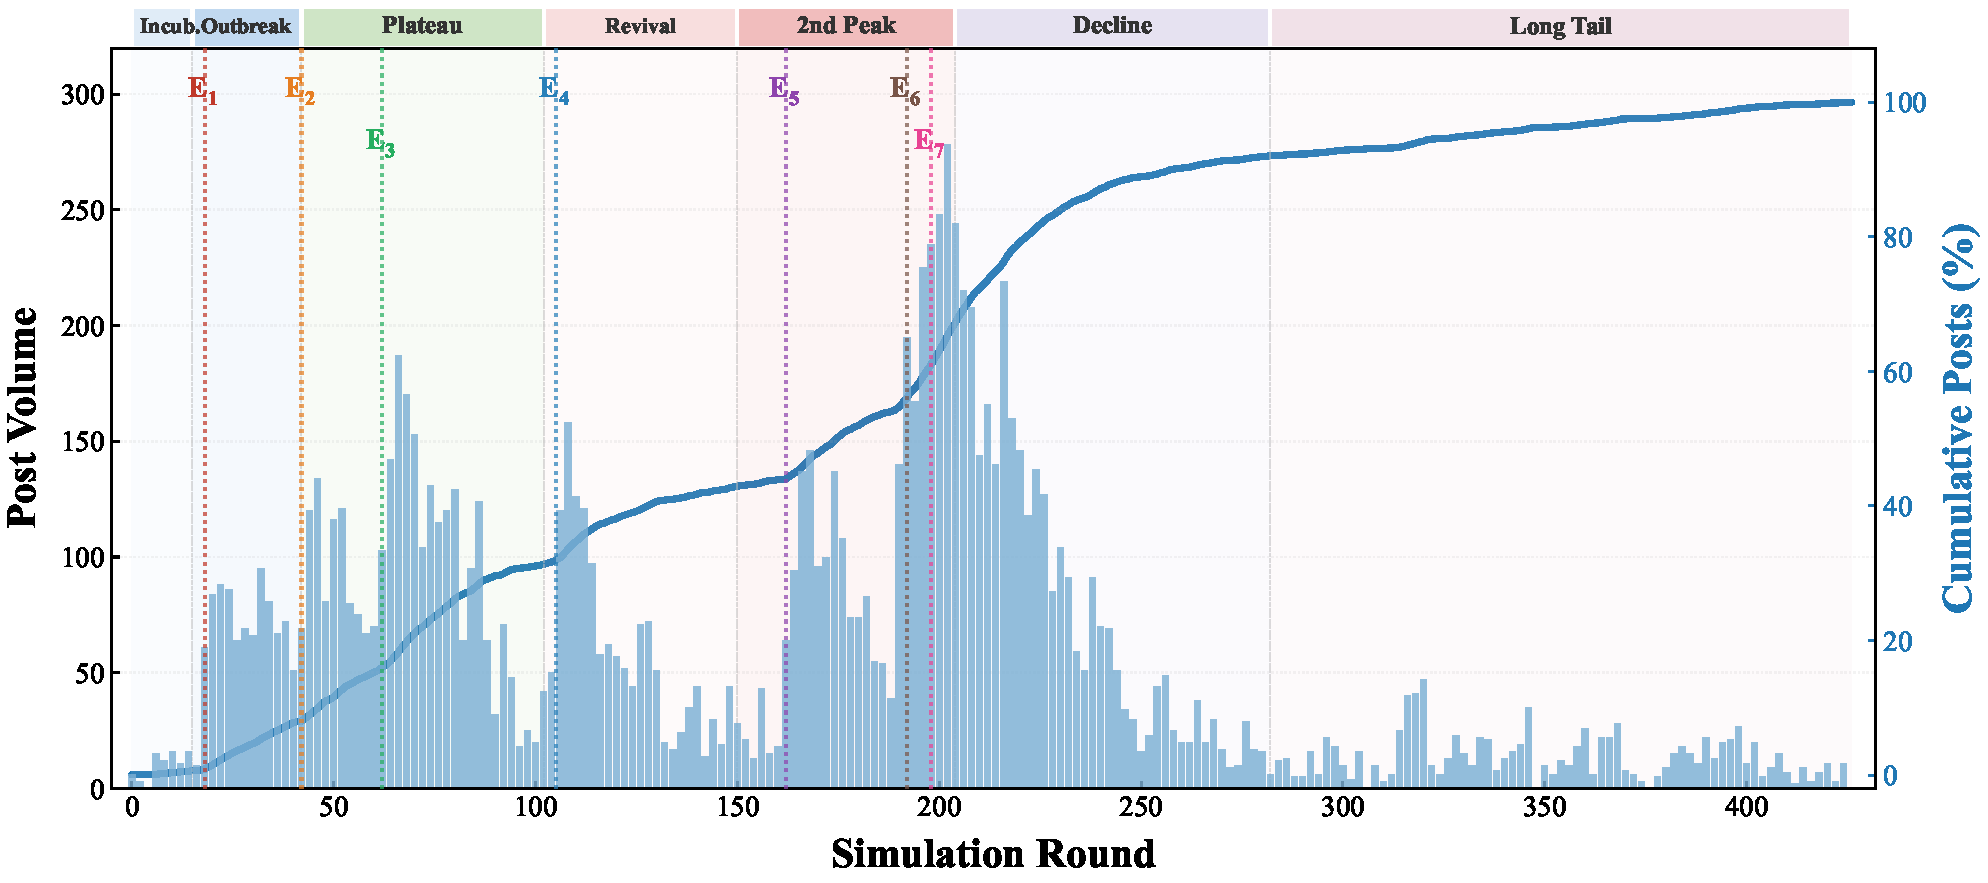
\includegraphics[width=0.82\textwidth]{fig_lifecycle_paper.pdf}
\caption{仿真舆情生命周期：发博量变化（柱状图，左轴）与累积发博百分比的观测S曲线（实线，右轴）及Logistic拟合曲线（虚线）。$E_1$--$E_7$标记外生事件注入时间点。}
\label{fig:lifecycle}
\end{figure}

如图~\ref{fig:lifecycle}所示，仿真清晰展现了西贝预制菜舆情事件从爆发、平台、复燃到衰退的多阶段生命周期~\citep{guo_stochastic_2024,chen_evolution_2025}，且各阶段转换均可溯源至特定事件的因果驱动。$E_1$（食品卫生视频曝光）注入后发博量迅速攀升，进入爆发期；$E_2$（罗永浩宣布停战）后活跃度明显回落，进入平台期；$E_4$（创始人群聊截图流出）重新点燃讨论，$E_5$（官媒发声点评）触发全程最大活跃度峰值，呈现典型的死灰复燃和官媒定调引发二次爆发的效应。累积发博百分比呈现S型增长曲线，与舆情传播学中S曲线扩散理论高度吻合~\citep{kong_exploring_2020}。值得强调的是，上述生命周期模式并非预设规则驱动，而是由霍克斯点过程的自激机制与智能体认知状态交互作用自发涌现的结果。在外生事件注入提升基础活跃智能体规模，而智能体发布的事件相关内容通过自激项$\sum \alpha e^{-\beta(t-t_i)}$进一步放大群体活跃度，形成正反馈的环路；当事件刺激消退且自激衰减后，活跃度自然回落。

\subsubsection{多主体行为异质性}

\begin{figure}[!t]
\centering
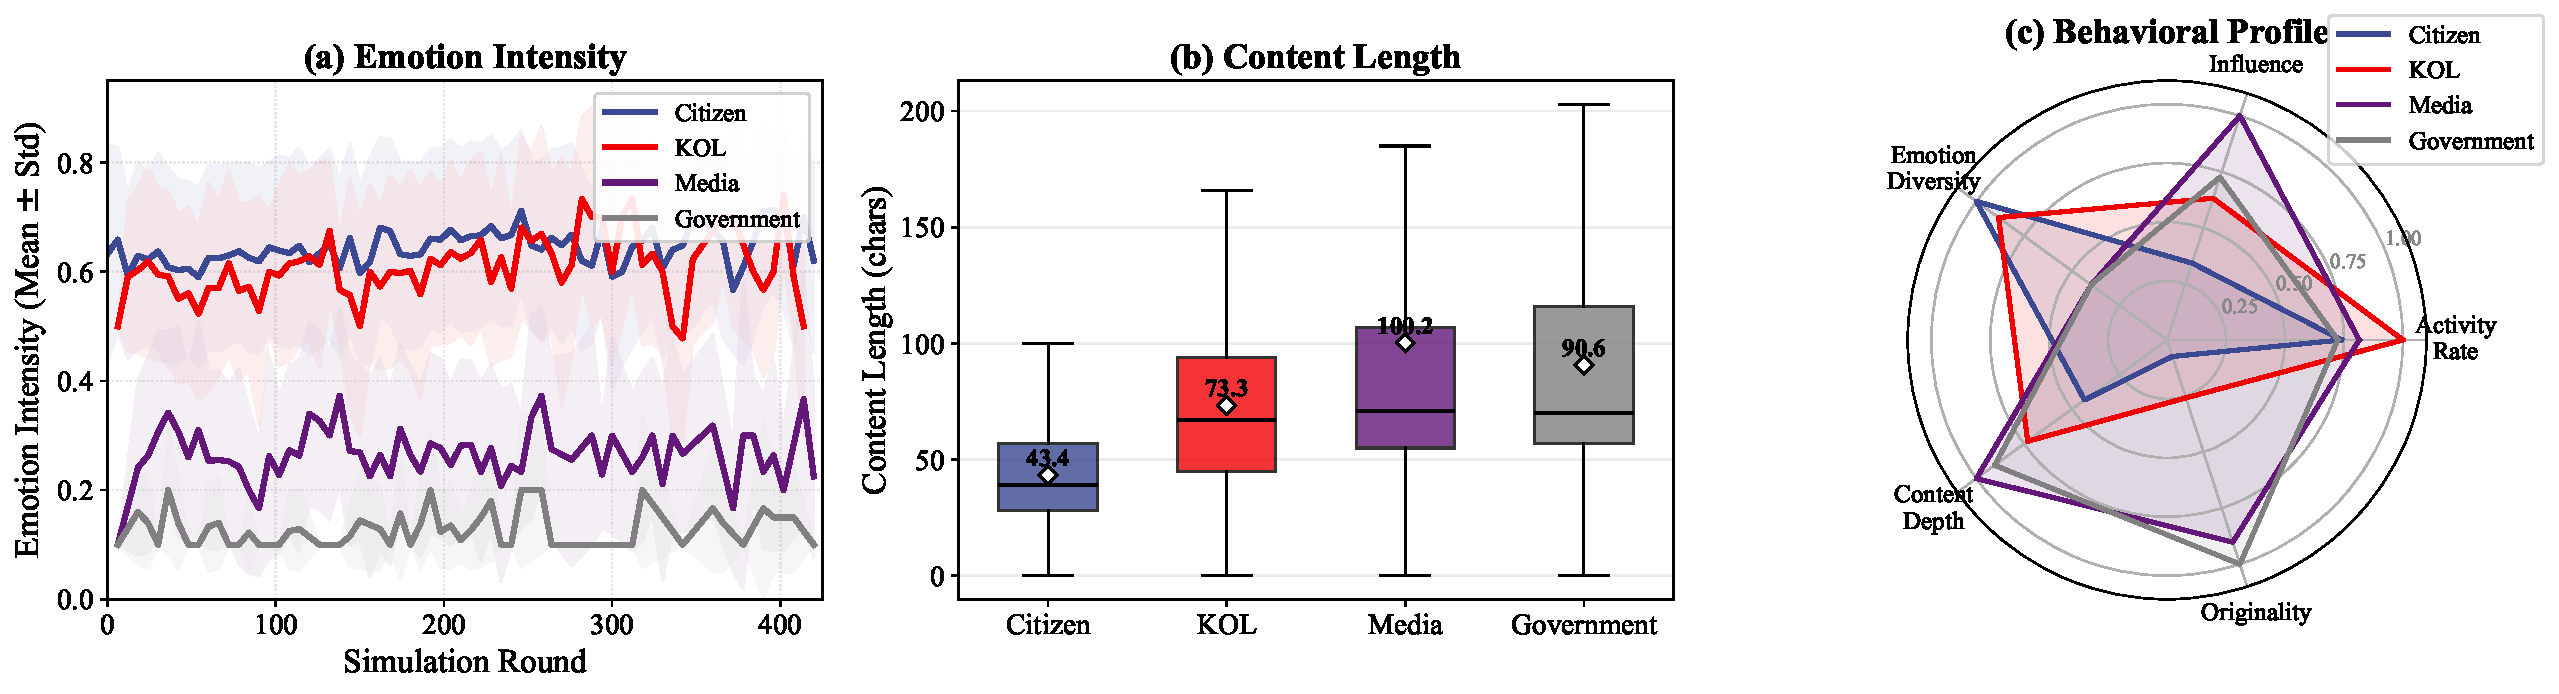
\includegraphics[width=\textwidth]{fig_paper_heterogeneity.pdf}
\caption{四类智能体行为异质性：(a)~情绪强度时序演化；(b)~内容长度分布；(c)~多维行为特征雷达图。}
\label{fig:heterogeneity}
\end{figure}

图~\ref{fig:heterogeneity}从情绪强度、内容长度和多维行为画像三个角度展示了四类智能体涌现出的系统性异质性。在情绪强度维度上，Citizen和KOL的平均情绪强度分别为0.645和0.603，始终处于高唤醒区间，且在事件刺激后呈现更剧烈的波动；Media和Government则稳定在低唤醒区间，呈现公众情绪化、官方中性化的分层模式，与真实舆情中“网民愤怒、官媒克制”的普遍观察一致。在内容长度维度上，Media和Government智能体的平均内容长度显著高于Citizen，反映了官方和媒体智能体生成更为详尽、结构化的内容输出。雷达图上四类智能体形成了形态截然不同的多边形：Citizen在情绪维度和互动频率上突出，KOL在影响力和内容产出量上领先，Media在内容质量和中性表达上占优，Government则以低频但高权威性的发言为特征。这些异质性模式并非手动编码，而是由EBDI架构中差异化的角色信念和动机权重自然涌现，验证了框架在多主体异质性建模上的有效性。

\subsubsection{情绪唤醒与极化效应}

基于情绪唤醒理论~\citep{berger_what_2012}和情绪传染假说~\citep{hatfield_emotional_1994}，我们从唤醒自增强和情绪传染两个维度进行验证（表~\ref{tab:emotion}）。

\begin{table}[!t]
\centering
\caption{Emotional arousal theory validation metrics.}
\label{tab:emotion}
\small
\renewcommand{\arraystretch}{1.1}
\begin{tabular}{@{}p{2.0cm}lcc@{}}
\toprule
\textbf{Dimension} & \textbf{Metric} & \textbf{Sim.\ Result} & \textbf{Theoretical Expectation} \\
\midrule
\multirow{3}{2.0cm}{Arousal Self-Reinforcement$^{\rm a}$}
 & High-arousal trend coeff.\ $\beta$ & $3.41{\times}10^{-4}$\,($p{<}.001$) & $\beta > 0$ \\
 & High-arousal emotion ratio & 73.5\% & Dominant \\
 & High/low arousal intensity ratio & 2.0$\times$ & $>1$ \\
\midrule
\multirow{2}{2.0cm}{Emotional Contagion$^{\rm b}$}
 & Comment-chain emotion consistency & 0.772 & $\gg$ random baseline \\
 & Escalation/de-escalation ratio & 4.78 & $>1$ (ratchet effect) \\
\bottomrule
\end{tabular}

\vspace{3pt}
{\footnotesize $^{\rm a}$~\citet{berger_what_2012};\quad $^{\rm b}$~\citet{hatfield_emotional_1994}}
\end{table}

高唤醒情绪占比随仿真推进呈显著上升趋势，总占比达73.5\%，与~\citet{berger_what_2012}所预测的正反馈机制一致。评论链情绪一致率高达0.772，升级/降级比为4.78，形成显著的棘轮效应，支持~\citet{hatfield_emotional_1994}的情绪传染假说。
与此同时，我们定义极化指数$\text{PI} = 1 - H/H_{\max}$。如图~\ref{fig:polarization}所示，极化指数从早期的0.41攀升至晚期的0.67（升幅63\%，$p < 0.001$），该趋势与回音室理论的预测一致~\citep{cinelli_echo_2021}。

\begin{figure}[!t]
\centering
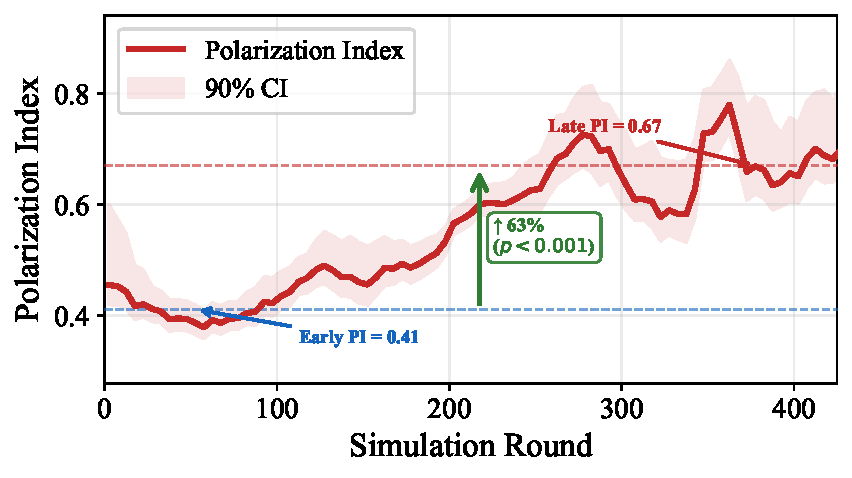
\includegraphics[width=0.65\columnwidth]{fig_paper_polarization.pdf}
\caption{情绪极化指数（PI）随仿真轮次的演化。实线为PI均值，阴影为90\% Bootstrap置信区间，虚线标注早期与晚期均值。}
\label{fig:polarization}
\end{figure}

\subsubsection{无标度拓扑与级联幂律}

\begin{figure}[!t]
\centering
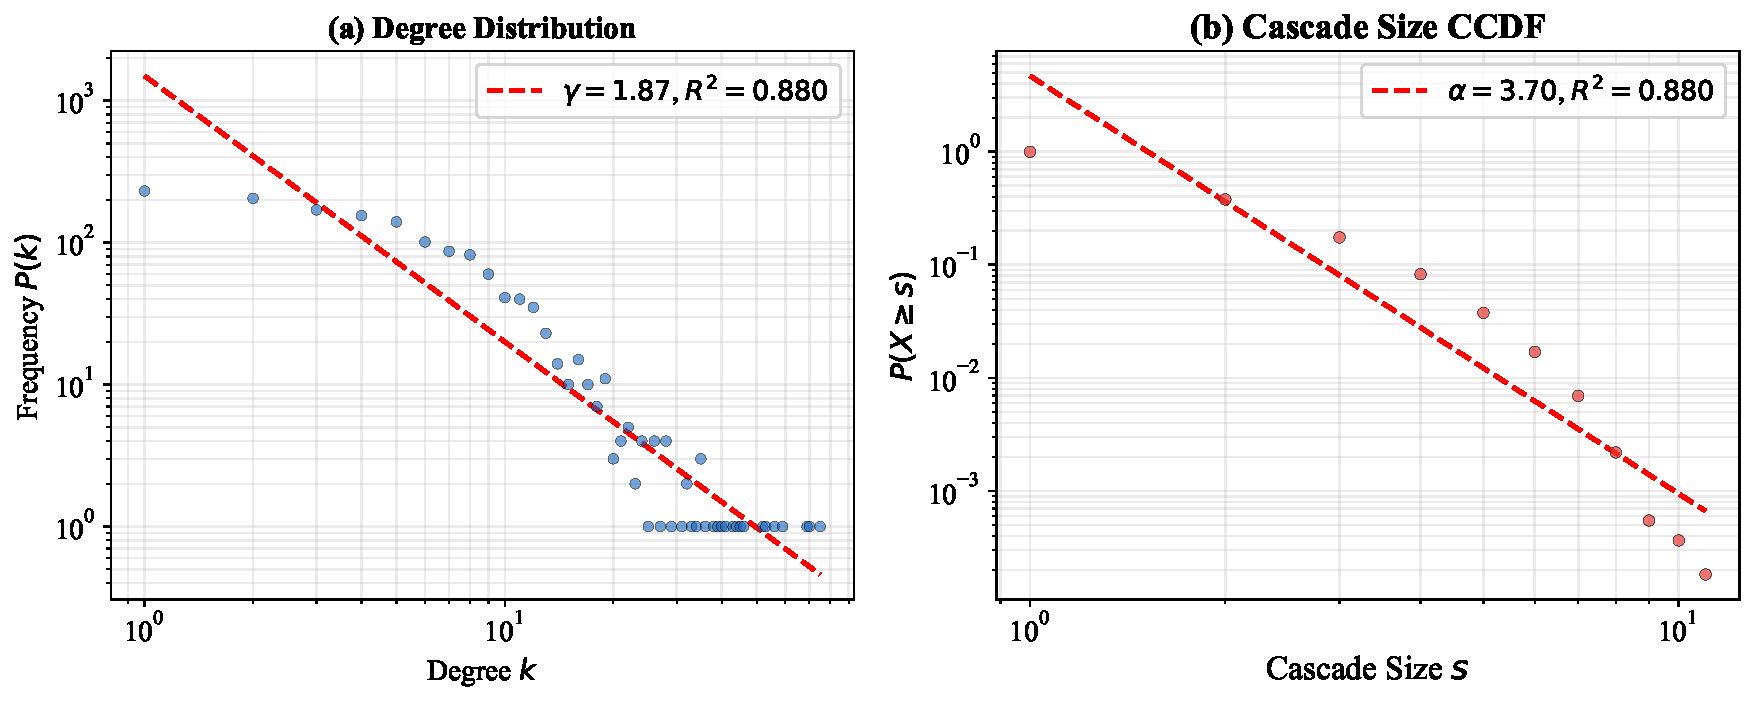
\includegraphics[width=0.75\textwidth]{fig_paper_powerlaw.pdf}
\caption{互动网络的拓扑特性：(a)~度分布幂律拟合$P(k) \sim k^{-\gamma}$；(b)~级联规模CCDF$P(X \geq s) \sim s^{-\alpha}$。}
\label{fig:powerlaw}
\end{figure}

真实社交网络的度分布和信息级联规模普遍服从幂律分布~\citep{barabasi_albert_1999}。如图~\ref{fig:powerlaw}(a)所示，互动网络的度分布幂律拟合指数$\gamma = 1.87$（$R^2 = 0.880$），落在真实社交网络中普遍报告的$1.5 < \gamma < 3$范围内，表明仿真网络呈现出典型的无标度特征——少数KOL和意见领袖节点形成高度数枢纽，而大量普通用户仅有少量连接。如图~\ref{fig:powerlaw}(b)所示，信息级联规模的互补累积分布函数（CCDF）拟合$\alpha = 3.70$（$R^2 = 0.880$），表明仿真中绝大多数转发级联规模较小，但偶尔出现涉及大量用户的爆发性传播，这与真实微博中“多数帖子无人问津、少数帖子病毒传播”的长尾现象一致。

\subsection{统计结果校准}

本节将仿真输出与三个真实舆情事件进行直接对比，从\textbf{行为层}（行为类型分布与活跃度曲线）、\textbf{内容层}（话语对抗性、词汇多样性与情感倾向）和\textbf{拓扑层}（网络结构与信息级联）三个维度进行系统性校准。

\subsubsection{对比方法}

统计校准关注大规模多智能体交互后涌现的群体行为是否在统计意义上与真实数据一致，因此对比方法需要在完整的仿真环境中运行端到端的多步仿真。设置三种对比基线：\textbf{Rule-based ABM}采用传统的规则驱动仿真，智能体的行为类型由基于身份的概率分布先验采样决定，整个决策过程不涉及LLM调用。\textbf{POSIM w/ LLM}在POSIM仿真环境下移除EBDI认知架构，智能体在接收推荐内容后直接由LLM单步生成行为决策和内容，不进行显式的信念更新或欲望推理。\textbf{POSIM w/ CoT}将EBDI的三阶段独立模块替换为单次思维链推理，在同一LLM调用中串联完成从认知到行为的全过程，保留POSIM的其他一切模式。

\subsubsection{评估指标}

评估从行为、内容和拓扑三个层面对仿真输出与真实数据进行定量比对，共计九个指标。

\textbf{行为层}度量智能体群体行为模式与真实用户的一致性，包含三个指标。行为类型分布散度BType JSD采用Jensen-Shannon散度衡量模拟与真实行为类型概率分布的差异，定义为：
\begin{equation}
\text{JSD}(P \| Q) = \tfrac{1}{2} D_{\text{KL}}(P \| M) + \tfrac{1}{2} D_{\text{KL}}(Q \| M)
\end{equation}
其中$M = (P + Q)/2$为两分布的均值分布。活跃度曲线Pearson相关系数Act.\,$\rho$衡量模拟与真实活跃度时序的线性相关性，活跃度曲线均方根误差Act.\,RMSE衡量两条曲线的绝对偏差。

\textbf{内容层}度量生成文本的语义特征与真实内容的匹配程度，包含三个指标。话语对抗性相似度Confr.\,Sim.基于关键词将话语分为对抗性、理性和中立三类，计算模拟与真实分布的相似度。词汇多样性偏差$|\Delta\text{TTR}|$衡量模拟与真实文本词汇丰富度的差异，其中TTR为Type-Token Ratio。情感均值偏差$|\Delta\bar{S}|$衡量群体情感倾向的整体偏移。

\textbf{拓扑层}度量仿真中涌现的网络结构与传播模式，包含三个指标。网络结构相似度Net.\,Sim.比较模拟与真实互动网络的拓扑特征，级联规模分布相似度Casc.\,Sim.比较信息级联规模的统计分布，级联幂律相似度Casc.\,PL比较级联规模幂律拟合参数的接近程度。

各层内的平均得分通过对越小越优的指标取$1{-}x$归一化后与越大越优的指标共同求均值得到。

\subsubsection{校准结果}

\begin{table}[!t]
\centering
\caption{Statistical calibration results across three events (LE\,=\,Luxury Earring, WL\,=\,WHU Library, XF\,=\,Xibei Prepared Food). \textbf{Bold}: best per dataset; \na: not applicable. \textcolor{gaingreen}{Green}: gain of POSIM over the second-best method.}
\label{tab:calibration}
\vspace{2pt}
\renewcommand{\arraystretch}{1.08}
\resizebox{\textwidth}{!}{%
\footnotesize
\begin{tabular}{@{}cl cccc cccc cccc@{}}
\toprule
\multirow{2}{*}{\textbf{Data}} & \multirow{2}{*}{\textbf{Method}}
& \multicolumn{4}{c}{\textbf{Behavior Layer}}
& \multicolumn{4}{c}{\textbf{Content Layer}}
& \multicolumn{4}{c}{\textbf{Topology Layer}} \\
\cmidrule(lr){3-6} \cmidrule(lr){7-10} \cmidrule(lr){11-14}
& & \makecell{BType\\JSD\,$\downarrow$} & \makecell{Act.\\$\rho$\,$\uparrow$} & \makecell{Act.\\RMSE\,$\downarrow$} & \makecell{Avg.\\$\uparrow$}
& \makecell{Confr.\\Sim.\,$\uparrow$} & \makecell{$|\Delta\text{TTR}|$\\$\downarrow$} & \makecell{$|\Delta\bar{S}|$\\$\downarrow$} & \makecell{Avg.\\$\uparrow$}
& \makecell{Net.\\Sim.\,$\uparrow$} & \makecell{Casc.\\Sim.\,$\uparrow$} & \makecell{Casc.\\PL\,$\uparrow$} & \makecell{Avg.\\$\uparrow$} \\
\midrule
\multirow{5}{*}{\textbf{LE}}
& Rule-based ABM        & 0.427 & 0.808 & 0.158 & 0.741 & \na & \na & \na & \na & 0.479 & 0.633 & 0.543 & 0.552 \\
& POSIM w/ LLM        & 0.289 & 0.799 & 0.162 & 0.783 & 0.544 & 0.185 & 0.319 & 0.680 & 0.565 & 0.735 & 0.918 & 0.739 \\
& POSIM w/ CoT          & 0.394 & 0.806 & \best{0.151} & 0.754 & 0.584 & 0.141 & 0.123 & 0.774 & 0.755 & 0.777 & 0.756 & 0.763 \\
\rowcolor{oursrow}
& \textbf{POSIM (Ours)}  & \best{0.193} & \best{0.809} & 0.154 & \best{0.821} & \best{0.790} & \best{0.030} & \best{0.029} & \best{0.910} & \best{0.895} & \best{0.830} & \best{0.961} & \best{0.896} \\[1pt]
\rowcolor{oursrow}
& & \gain{+.096} & \gain{+.001} & \gain{+.000} & \gain{+.038} & \gain{+.206} & \gain{+.111} & \gain{+.094} & \gain{+.136} & \gain{+.140} & \gain{+.053} & \gain{+.043} & \gain{+.133} \\
\midrule
\multirow{5}{*}{\textbf{WL}}
& Rule-based ABM        & 0.318 & 0.681 & 0.126 & 0.746 & \na & \na & \na & \na & 0.869 & 0.696 & 0.642 & 0.736 \\
& POSIM w/ LLM        & 0.237 & 0.722 & 0.119 & 0.789 & 0.453 & 0.172 & 0.360 & 0.640 & 0.528 & 0.667 & 0.580 & 0.592 \\
& POSIM w/ CoT          & 0.229 & 0.744 & \best{0.116} & 0.800 & 0.474 & 0.091 & 0.365 & 0.673 & \best{0.941} & 0.740 & 0.673 & 0.784 \\
\rowcolor{oursrow}
& \textbf{POSIM (Ours)}  & \best{0.073} & \best{0.750} & 0.118 & \best{0.853} & \best{0.841} & \best{0.010} & \best{0.203} & \best{0.876} & 0.850 & \best{0.758} & \best{0.965} & \best{0.858} \\[1pt]
\rowcolor{oursrow}
& & \gain{+.156} & \gain{+.006} & \gain{+.000} & \gain{+.053} & \gain{+.367} & \gain{+.081} & \gain{+.157} & \gain{+.203} & \gain{+.000} & \gain{+.018} & \gain{+.292} & \gain{+.074} \\
\midrule
\multirow{5}{*}{\textbf{XF}}
& Rule-based ABM        & 0.312 & 0.664 & 0.187 & 0.721 & \na & \na & \na & \na & 0.528 & 0.614 & 0.279 & 0.474 \\
& POSIM w/ LLM        & 0.244 & 0.671 & 0.190 & 0.746 & 0.765 & 0.117 & 0.076 & 0.858 & 0.774 & 0.695 & 0.482 & 0.650 \\
& POSIM w/ CoT          & 0.293 & 0.699 & 0.181 & 0.742 & 0.774 & 0.134 & \best{0.014} & 0.875 & 0.767 & 0.696 & 0.460 & 0.641 \\
\rowcolor{oursrow}
& \textbf{POSIM (Ours)}  & \best{0.148} & \best{0.727} & \best{0.168} & \best{0.804} & \best{0.843} & \best{0.019} & 0.046 & \best{0.926} & \best{0.885} & \best{0.696} & \best{0.513} & \best{0.698} \\[1pt]
\rowcolor{oursrow}
& & \gain{+.096} & \gain{+.028} & \gain{+.013} & \gain{+.058} & \gain{+.069} & \gain{+.098} & \gain{+.000} & \gain{+.051} & \gain{+.111} & \gain{+.000} & \gain{+.031} & \gain{+.048} \\
\bottomrule
\end{tabular}%
}
\end{table}

实验在三个真实舆情数据集上开展，结果如表~\ref{tab:calibration}所示（三个事件的统计校准可视化详见附录图~\ref{fig:three_event_calibration}）。

\textbf{行为层校准。}POSIM在三个数据集上的BType JSD均取得最优，说明EBDI元认知架构产生的行为决策在类型比例上与真实数据高度一致。值得注意的是，WL数据集的JSD仅为0.073，远优于其他方法，这与该事件中校园讨论的行为模式相对集中有关，EBDI的信念锚定机制使智能体能够准确捕捉这种集中趋势。仅使用LLM单步决策（POSIM w/ LLM）时，行为分布偏差显著增大，尤其在LE和XF数据集上JSD分别达到0.289和0.244，表明缺乏分层认知约束的LLM倾向于产生行为类型趋同。热度时序相关性$\rho$方面，POSIM在三个数据集上均保持高相关度，表明霍克斯点过程驱动的时间引擎有效捕捉了舆情活跃度的时序波动模式。行为层平均得分在三个数据集上分别达到0.821、0.853和0.804，跨事件类型的稳定表现证明了框架的通用性。

\textbf{内容层校准。}POSIM的对抗性相似度在所有数据集上均最高，表明EBDI架构能够准确再现舆情中理性与对抗性话语的分布格局。相比之下，POSIM w/ LLM的对抗性相似度仅为0.423--0.774，差距在LE数据集上尤为显著（0.790 vs. 0.423），原因在于天价耳环事件中公众情绪对抗性强烈，缺乏欲望模块的动机约束使LLM生成的内容倾向于中性化表达，无法再现真实舆情中的话语对抗格局。词汇多样性差异$|\Delta\text{TTR}|$在所有数据集上同样最小，表明分层认知推理中信念模块维护的个性化角色信息有效避免了LLM的平均人格问题，使不同智能体产生了具有个人风格的差异化文本。情感偏差$|\Delta\bar{S}|$方面，POSIM在所有数据集上均保持极低水平，说明EBDI中情绪因素的显式建模使仿真内容的整体情感倾向与真实数据高度吻合。内容层平均得分在三个数据集上分别为0.910、0.876和0.926。

\textbf{拓扑层校准。}评估采用内容来源链追踪机制，POSIM在三个数据集上均取得最优的拓扑层平均得分。在网络相似度维度上，POSIM在LE和XF数据集上分别达到0.895和0.885，显著优于Rule-based ABM的0.479和0.528，表明EBDI的多级意图规划使智能体能够基于内容质量和社交亲和度做出有区分度的交互选择，从而涌现出更接近真实的网络拓扑。在级联幂律维度上，差异更为显著：POSIM在LE数据集上达到0.961，而Rule-based ABM仅为0.543，说明随机交互决策无法产生真实社交网络中的长尾级联分布。XF数据集的拓扑层平均得分相对较低，可能与该事件持续时间较长、网络结构更为复杂有关，但POSIM仍显著优于所有基线方法。

\textbf{综合分析。}POSIM在三个层面均全面领先，核心优势源于EBDI架构的分层认知设计：信念子系统为行为决策提供个性化的认知锚定，欲望子系统通过动机约束驱动对抗性话语的准确再现，意图子系统的结构化分解保障了词汇多样性和交互拓扑的合理性。三个基线的表现差异也佐证了这一判断——Rule-based ABM因缺乏认知驱动而在拓扑层表现最差，POSIM w/ LLM因缺少信念锚定而在内容层一致性不足，POSIM w/ CoT因模块间缺乏独立约束而整体居中。

\vspace{6pt}
\subsection{消融实验}

为验证POSIM各核心模块的必要性，设置完整框架与若干变体配置进行对比。\textbf{Full POSIM}为包含所有模块的完整框架。\textbf{w/o Belief}移除信念更新模块，智能体不维护显式的信念状态，欲望和意图直接基于当前感知信息生成，不参考历史认知积累。\textbf{w/o Desire}移除欲望生成模块，意图规划不再接收动机权重约束，LLM直接从信念状态生成行为决策，缺失了动机层面的中间推理。\textbf{w/o Intention}移除意图规划模块，行为决策不再经过三级思维链的结构化分解（行为选择、表达策略规划和内容生成），LLM直接从信念和欲望状态生成最终行为输出，缺失了表达策略层面的显式约束。\textbf{w/o Hawkes}将霍克斯点过程时间引擎替换为固定时间步长的均匀激活模式，每步激活固定数量的智能体，移除了事件驱动的动态时间调度机制。结果如表~\ref{tab:ablation}所示。

\begin{table}[!t]
\centering
\caption{Ablation study results (LE dataset). \underline{Underline} marks cases where a variant outperforms the full model.}
\label{tab:ablation}
\small
\renewcommand{\arraystretch}{1.05}
\begin{tabular}{@{}l ccc ccc cc@{}}
\toprule
\multirow{2}{*}{\textbf{Configuration}} & \multicolumn{3}{c}{\textbf{Behavior Layer}} & \multicolumn{3}{c}{\textbf{Content Layer}} & \multicolumn{2}{c}{\textbf{Topology Layer}} \\
\cmidrule(lr){2-4} \cmidrule(lr){5-7} \cmidrule(lr){8-9}
& \makecell{JSD\\$\downarrow$} & \makecell{$\rho$\\$\uparrow$} & \makecell{RMSE\\$\downarrow$}
& \makecell{Confr.\\$\uparrow$} & \makecell{$|\Delta$TTR$|$\\$\downarrow$} & \makecell{$|\Delta\bar{S}|$\\$\downarrow$}
& \makecell{Net.\\$\uparrow$} & \makecell{Casc.\\$\uparrow$} \\
\midrule
\rowcolor{greenrow}
Full POSIM & \best{0.193} & \best{0.809} & \best{0.154} & \best{0.790} & \best{0.030} & \best{0.029} & \best{0.895} & \best{0.830} \\
w/o Belief & 0.258 & 0.762 & 0.172 & 0.706 & 0.058 & 0.067 & 0.861 & 0.773 \\
w/o Desire & 0.267 & 0.779 & 0.169 & 0.682 & 0.071 & 0.083 & 0.853 & 0.788 \\
w/o Intention & 0.237 & 0.802 & 0.159 & 0.728 & 0.064 & 0.055 & 0.858 & 0.814 \\
w/o Hawkes & \underline{0.177} & 0.235 & 0.362 & 0.787 & 0.207 & \underline{0.028} & 0.822 & 0.754 \\
\bottomrule
\end{tabular}
\end{table}

\textbf{w/o Hawkes}移除霍克斯点过程后，$\rho$从0.809骤降至0.235，RMSE从0.154恶化至0.362，表明均匀激活模式无法捕捉舆情活跃度的时序波动。其BType JSD（0.177）略优于Full POSIM（0.193），这是因为均匀激活下行为类型分布因大数定律趋于均匀，但丧失了事件驱动的活跃度突变特征。$|\Delta\text{TTR}|$恶化至0.207，说明时间引擎异常间接导致内容同质化。

\textbf{w/o Belief}移除信念模块后各指标普遍下降：JSD恶化至0.258，对抗性相似度从0.790降至0.706，$|\Delta\bar{S}|$恶化至0.067。信念模块维护的$B^{evt}$和$B^{emo}$是生成对抗性话语的核心依据，其缺失导致智能体丧失对争议焦点的深层理解。

\textbf{w/o Desire}移除欲望模块后内容层退化最严重：对抗性相似度降至0.682（所有变体最低），$|\Delta\bar{S}|$恶化至0.083（最大），表明动机类型是驱动激烈话语表达的核心因素，缺失后LLM倾向于生成中性化文本。

\textbf{w/o Intention}移除意图模块后，$|\Delta\text{TTR}|$恶化至0.064（最严重），网络相似度降幅最大（$\Delta=-3.7$pp），说明三级思维链的结构化分解对词汇多样性和交互拓扑至关重要。

\textbf{综合分析。}四组消融实验表明各组件具有清晰的功能分工：信念子系统提供全局认知支撑，欲望子系统驱动内容层的对抗性表达，意图子系统保障词汇多样性和交互拓扑，霍克斯引擎决定时序一致性，验证了EBDI分层架构各组件的互补性。

% ============================================================
% 第6节 案例研究
% ============================================================
\section{案例研究}\label{sec:case}

POSIM的模块化架构使其具备向多种应用场景扩展的能力。本节通过两项案例研究展示框架作为计算实验平台的应用价值：认知引导实验探索不同认知干预策略对群体情绪的调控效果，反事实策略评估对比不同公关策略在危机事件中的效果差异。

\subsection{认知引导实验}

基于天价耳环事件设计认知引导实验，200个智能体仿真30步，在第5步对随机选取的智能体注入认知引导，分别测试30\%、60\%和100\%三种覆盖率。对照组保持无干预基线，三种干预策略分别对应不同的认知调控机制。\textbf{理性认知引导}（RC）引导智能体从多角度理性分析事件，\textbf{共情引导}（EP）鼓励理解当事人立场，\textbf{情绪调节}（ER）引导智能体识别和管理自身情绪。结果如表~\ref{tab:priming}所示。

\begin{table}[!t]
\centering
\caption{Cognitive priming experiment results (200 agents, 30 steps). Coverage denotes the proportion of agents receiving cognitive priming.}
\label{tab:priming}
\small
\renewcommand{\arraystretch}{1.05}
\begin{tabular}{@{}llccc@{}}
\toprule
\textbf{Condition} & \textbf{Coverage} & \makecell{\textbf{Neg.\ Emotion}\\\textbf{Ratio}\,$\downarrow$} & \makecell{\textbf{Anger}\\\textbf{Ratio}\,$\downarrow$} & \makecell{\textbf{Emotion}\\\textbf{Intensity}\,$\downarrow$} \\
\midrule
Control & --- & 0.844 & 0.600 & 0.649 \\
\midrule
\multirow{3}{*}{\makecell[l]{Rational\\Cognition (RC)}}
 & 30\% & 0.767 & 0.534 & 0.621 \\
 & 60\% & 0.753 & 0.506 & 0.595 \\
 & 100\% & \best{0.571} & \best{0.407} & \best{0.527} \\
\midrule
\multirow{3}{*}{\makecell[l]{Empathy\\Priming (EP)}}
 & 30\% & 0.794 & 0.523 & 0.609 \\
 & 60\% & 0.806 & 0.535 & 0.617 \\
 & 100\% & 0.878 & 0.569 & 0.650 \\
\midrule
\multirow{3}{*}{\makecell[l]{Emotional\\Regulation (ER)}}
 & 30\% & 0.831 & 0.583 & 0.626 \\
 & 60\% & 0.644 & 0.503 & 0.587 \\
 & 100\% & 0.572 & 0.481 & 0.573 \\
\bottomrule
\end{tabular}
\end{table}

\begin{figure}[!t]
\centering
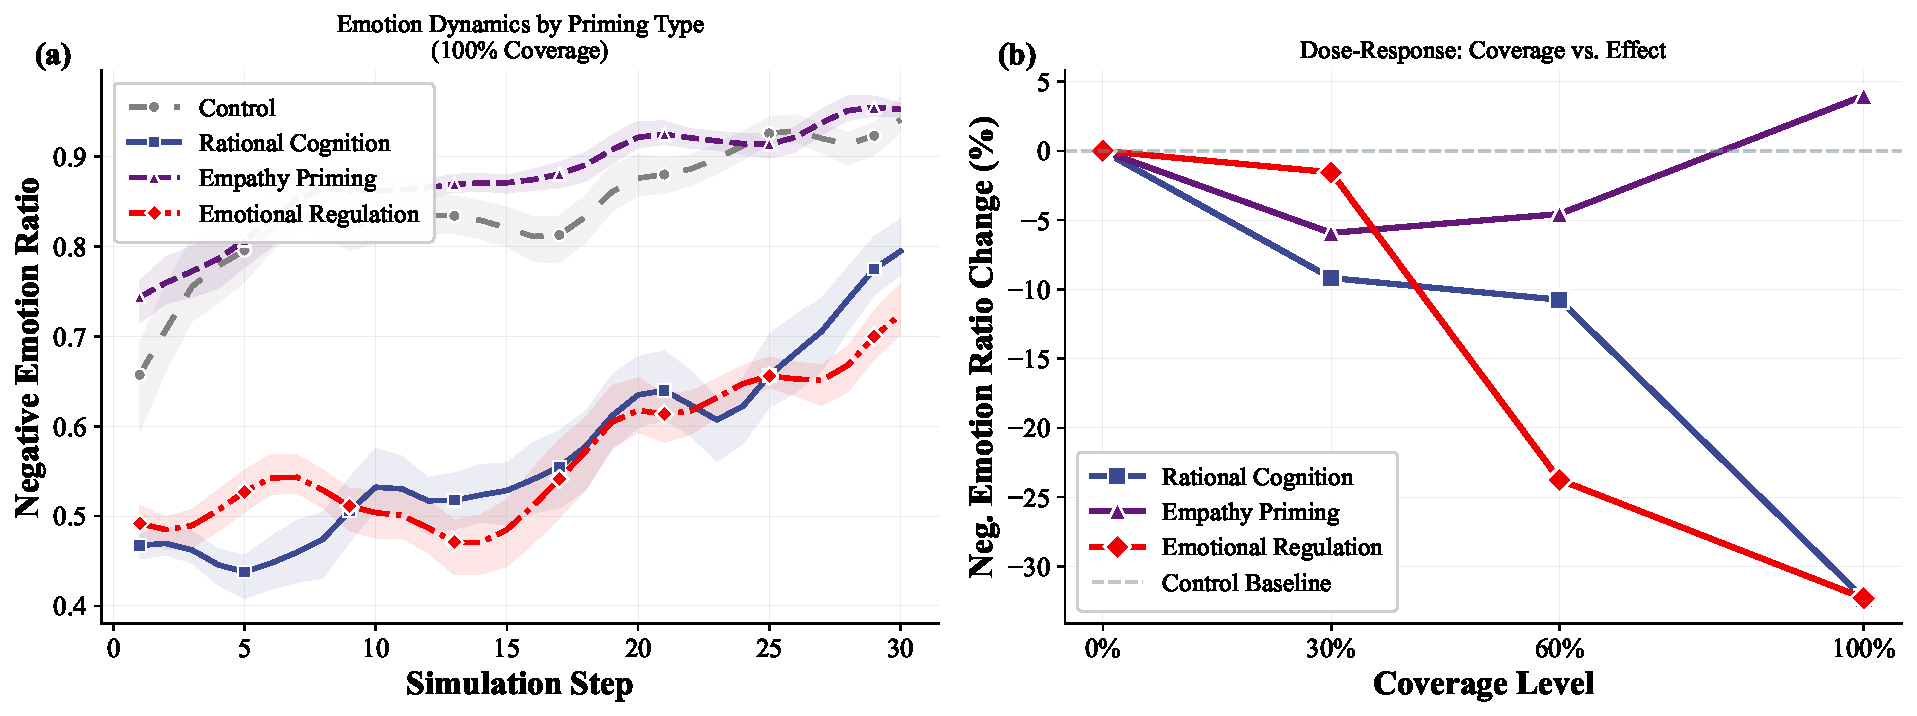
\includegraphics[width=0.95\textwidth]{paper_cognitive_priming.pdf}
\caption{认知引导实验：(a)~100\%覆盖率下四种条件的NER时序演化；(b)~三种策略的NER变化幅度随覆盖率的剂量-效应关系。}
\label{fig:priming}
\end{figure}

实验揭示了三个关键发现。RC和ER策略显著降低负面情绪且呈现剂量效应，如图~\ref{fig:priming}所示，RC将负面情绪比例从0.844降至0.571（降幅32.3\%），图~\ref{fig:priming}(b)显示RC的覆盖率跨越60\%后效果显著跃升，呈现阈值效应。EP的负面情绪比例为0.878，反而高于对照组的0.844，且随覆盖率增大反而上升，呈现反剂量效应。这一共情悖论在社会心理学中已有理论预期~\citep{batson_empathy_1991}，共情理解他人痛苦的同时会产生更多移情性负面情绪，在仿真中首次被定量观察到。各条件下的行为总量高度一致，变异系数仅4.6\%，表明EBDI架构实现了行为动机与情绪表达的有效解耦。

\subsection{反事实策略评估}

基于西贝预制菜事件设计反事实实验，保持外部事件不变，仅替换西贝的公关响应，比较五种策略。\textbf{实际应对}（AR）复现了西贝从强硬否认到辱骂再到秒删致歉的真实应对过程，\textbf{及时致歉}（SEA）在事件初期即发布诚恳致歉声明，\textbf{主动透明}（PT）主动公开预制菜使用信息和食品安全报告，\textbf{消费者对话}（CD）直接与消费者进行互动和沟通，\textbf{战略沉默}（SS）对事件不做任何公开回应。每种策略使用200个智能体、20步仿真，策略在舆情爆发初期和中期各部署一次。结果见表~\ref{tab:counter}。

\begin{table}[!t]
\centering
\caption{Counterfactual strategy evaluation results (200 agents, 20 steps).}
\label{tab:counter}
\small
\renewcommand{\arraystretch}{1.05}
\begin{tabular}{@{}lccc@{}}
\toprule
\textbf{Strategy} & \makecell{\textbf{Neg.\ Emotion}\\\textbf{Ratio}\,$\downarrow$} & \makecell{\textbf{Anger}\\\textbf{Ratio}\,$\downarrow$} & \makecell{\textbf{Emotion}\\\textbf{Intensity}\,$\downarrow$} \\
\midrule
Actual Response (AR) & 0.792 & 0.791 & 0.685 \\
Swift Early Apology (SEA) & 0.749 & 0.749 & 0.612 \\
Proactive Transparency (PT) & 0.773 & 0.773 & 0.645 \\
\rowcolor{greenrow}
Consumer Dialogue (CD) & \best{0.744} & \best{0.743} & \best{0.598} \\
Strategic Silence (SS) & 0.831 & 0.831 & 0.702 \\
\bottomrule
\end{tabular}
\end{table}

实验揭示了三个关键发现。积极策略显著优于消极应对，CD策略效果最优，SEA次之（NER为0.749），PT第三（0.773）。战略沉默表现最差，沉默策略仅对30\%的智能体产生轻微信念修正，绝大多数智能体的事件观点信念维持原始负面状态，验证了危机公关中沉默并非最优选择的教训。策略效果呈即时降温与逐步反弹的动态模式，时序分析显示SEA在部署后NER一度降至0.56，但随后在负面内容推荐的持续作用下逐步回升，精确模拟了真实舆情中公关效果衰减的常见现象。策略传导严格遵循信念修正、认知推理改变、行为输出转变的因果链条，验证了EBDI架构在策略评估中的可解释性优势。

% ============================================================
% 第7节 讨论（IPM要求）
% ============================================================
\section{结果讨论与启示}\label{sec:discussion}

\subsection{主要发现}

本研究通过三层递进验证体系对POSIM框架进行了系统性评估，获得了以下主要发现。

在微观行为机制层面，EBDI元认知架构在认知行为链一致性（4.64/5.0）、人格稳定性（0.661）和决策抗扰性（0.695）三项指标上全面优于直接提示和思维链方法。这一结果表明，将LLM嵌入分层认知架构并赋予智能体显式的信念、欲望和意图状态，能够有效提升行为决策的认知深度和可解释性。特别值得注意的是，CoT方法虽然在认知链一致性上优于Direct方法，但其决策抗扰性反而最低（0.541），原因在于思维链推理在单次调用中缺乏稳定的状态锚定，容易受输入扰动的影响。EBDI通过显式的信念状态和欲望系统提供了认知锚定效应，使决策在面对输入变化时保持更高的稳定性。

在宏观涌现层面，仿真系统在无任何宏观层面的显式编程的情况下，自发涌现出了与社会科学理论一致的多种宏观现象，包括事件驱动的多阶段生命周期、四类智能体的系统性行为异质性、情绪唤醒自增强与极化效应（极化指数从0.41上升至0.67）、以及无标度网络拓扑（$\gamma=1.87$）和级联幂律分布（$\alpha=3.70$）。这些涌现现象为POSIM的理论有效性提供了强有力的佐证，表明微观层面精确的认知建模能够在宏观层面产生符合社会科学规律的集体行为。

在统计校准层面，POSIM在三个数据集上的行为层、内容层和拓扑层均全面优于基线方法，模拟结果的行为、内容和拓扑指标相较于最优基线分别提升了\textbf{5.0\%}、\textbf{13.0\%}和\textbf{8.5\%}。消融实验进一步表明各认知子系统具有清晰的功能分工与互补性，其中欲望子系统对内容层的对抗性话语再现贡献最为显著，信念子系统为行为层的个性化决策提供了不可替代的认知锚定。

\subsection{理论启示}

在智能体建模层面，EBDI架构将大语言模型与经典BDI认知框架相融合，为人工社会仿真提供了一种兼具认知深度与行为多样性的设计范式。区别于现有端到端LLM智能体将决策过程视为黑箱，EBDI通过显式的认知状态分层和多阶段决策链，使智能体的行为输出不仅在结果上贴近真实网民，在生成过程上也具备认知科学意义上的可解释性，这一范式有望推广至更广泛的社会仿真场景。

在评估方法论层面，本文构建的三层递进验证体系——微观机制校准、宏观涌现校准与统计一致性校准——分别对应仿真系统的内部有效性、构念有效性和外部有效性，形成从机制到现象再到数据的完整验证链条，可为后续基于LLM的社会仿真研究提供可复用的评估参考。

在应用扩展层面，两项案例研究从不同角度展示了框架的计算实验能力。认知引导实验中观察到的共情悖论效应~\citep{batson_empathy_1991}表明，仿真系统能够捕捉认知科学中细微的非线性机制，而非简单地再现引导即改善的线性因果；反事实策略评估则验证了框架在危机公关决策支持中的实用价值。这些结果共同表明，POSIM已超越单纯的仿真工具定位，具备向多元舆情治理场景扩展的计算实验平台潜力。

\subsection{实践启示}

从危机公关实践角度看，反事实策略评估实验揭示了两条值得关注的规律。其一，主动沟通类策略在降低负面情绪方面显著优于消极应对，消费者对话策略效果最优而战略沉默效果最差——这一结论虽与危机公关理论的既有预期吻合，但在本研究中首次获得了基于大规模智能体仿真的定量支撑。其二，策略效果并非一成不变，而是呈现即时降温与逐步反弹的动态模式，揭示出信念修正具有时效性，提示决策者在部署公关策略后仍需持续关注后续舆情走势。

认知引导实验则为舆情治理中的资源配置提供了量化参考：理性认知引导策略在覆盖率跨越60\%后效果显著跃升，呈现清晰的阈值效应，意味着有限资源下精准覆盖关键人群可能比广撒网式干预更为高效。

\subsection{局限性}

尽管实验结果整体积极，本研究仍存在若干不足。首先，框架的认知推理质量与底层LLM的能力紧密耦合，更换模型可能带来不同的仿真表现，大规模仿真的推理成本也仍有压缩空间。其次，当前社交网络中的关注关系在仿真过程中保持静态，尚未纳入用户间关注与取关的动态演化机制。再者，实验验证仅覆盖微博平台的三个事件，框架在不同社交媒体平台和文化语境下的迁移能力有待进一步考察。此外，微观层面部分评估指标依赖LLM作为评判者，可能引入系统性偏差；消融实验目前仅在天价耳环数据集上完成，跨事件类型的一致性验证尚需补充。

% ============================================================
% 第8节 结论
% ============================================================
\section{结论}\label{sec:conclusion}

本文提出了社交媒体舆情仿真框架POSIM，其核心思路是将大语言模型嵌入EBDI分层认知架构以构建元认知智能体，并以霍克斯自激点过程统一建模外生事件冲击与内生用户交互，从而在分钟级时间分辨率下实现高精度的舆情演化仿真。

三层递进验证的实验结果支撑了以下结论。在微观层面，EBDI架构在认知行为链一致性、人格稳定性和决策抗扰性上全面优于直接提示与思维链方法，证实了分层独立认知建模相较于端到端生成的系统性优势。在宏观层面，仿真系统在无显式宏观编程的条件下自发涌现出舆情生命周期、情绪极化、无标度拓扑和级联幂律等与社会科学理论一致的集体行为模式。在统计校准层面，POSIM的行为、内容和拓扑指标相较于最优基线分别提升了5.0\%、13.0\%和8.5\%，跨事件类型的稳健表现验证了框架的通用性。此外，两项案例研究展示了框架向认知干预和反事实策略评估等应用场景扩展的能力，表明POSIM不仅是一个仿真器，更具备作为舆情治理计算实验平台的潜力。

未来工作将在以下方向展开：引入动态社交网络建模以刻画关注关系的演化，拓展至多平台多语言的舆情场景，探索更高效的LLM调用与推理加速策略，并将框架应用于更多样化的社会仿真任务。

% ============================================================
% 参考文献
% ============================================================
\bibliographystyle{model5-names}
\bibliography{posim_refs}

% ============================================================
% 附录
% ============================================================
\appendix

% ============================================================
% 附录A：核心算法伪代码
% ============================================================
\section{核心算法伪代码}

\noindent
\begin{minipage}[t]{0.48\textwidth}
\begin{algorithm}[H]
\caption{POSIM仿真主循环}
\label{alg:main}
\begin{algorithmic}[1]
\REQUIRE 智能体集合$\mathcal{U}$，事件队列$\mathcal{E}$，配置$\mathcal{C}$
\ENSURE 仿真轨迹$\mathcal{T}$
\STATE 初始化霍克斯过程$\mathcal{H}$
\STATE 初始化推荐系统$\mathcal{R}$和热搜系统$\mathcal{S}$
\FOR{$t = 0, 1, \ldots, T_{max}$}
 \STATE $t_{sim} \leftarrow t_0 + t \cdot \Delta t$
 \STATE $\mathcal{E}_{cur} \leftarrow \mathcal{E}.\text{get\_events}(t_{sim})$
 \FORALL{$e \in \mathcal{E}_{cur}$}
 \STATE $\mathcal{H}.\text{add\_ext}(t, e.\text{inf})$
 \ENDFOR
 \STATE 计算$\lambda_{adj}(t)$（式\ref{eq:hawkes}）
 \STATE $N_t \!\leftarrow\! \text{Poisson}(\lambda_{adj} \!\cdot\! N_{s} \!\cdot\! \Delta t / 60)$
 \STATE $\mathcal{A}_t \leftarrow \text{WSample}(\mathcal{U}, N_t)$
 \FORALL{$u \in \mathcal{A}_t$ \textbf{parallel}}
 \STATE $P_t \leftarrow \mathcal{R}.\text{rec}(u, t_{sim})$
 \STATE $I_u \leftarrow \text{EBDI}(u, P_t, \mathcal{E}_{ctx})$
 \STATE 执行$I_u$并更新$\mathcal{H}$
 \ENDFOR
 \STATE 情绪传染；更新热搜$\mathcal{S}$
 \STATE $\mathcal{T} \leftarrow \mathcal{T} \cup \{(t, \mathcal{A}_t, I)\}$
\ENDFOR
\RETURN $\mathcal{T}$
\end{algorithmic}
\end{algorithm}
\end{minipage}
\hfill
\begin{minipage}[t]{0.48\textwidth}
\begin{algorithm}[H]
\caption{EBDI认知决策管线}
\label{alg:ebdi}
\begin{algorithmic}[1]
\REQUIRE 智能体$u$，感知$P_t$，事件$\mathcal{E}_{ctx}$
\ENSURE 行为序列$I_t$
\STATE \textbf{阶段1：信念更新}
\STATE $M_t \leftarrow \text{Memory.get}(P_t, k)$
\STATE $B_t \leftarrow f_{\text{LLM}}(B_{t-1}, P_t, M_t, \Phi)$
\STATE $B_t.\text{emo} \leftarrow B_t.\text{emo} \odot e^{-\lambda_e \Delta t}$
\STATE \textbf{阶段2：欲望生成}
\STATE $D_t \leftarrow g_{\text{LLM}}(B_t, P_t)$
\STATE \textbf{阶段3：意图规划}
\STATE $L_1 \leftarrow \text{SelectAction}(B_t, D_t, P_t)$
\STATE $L_2 \leftarrow \text{PlanStrategy}(L_1, B_t)$
\STATE $L_3 \leftarrow \text{GenContent}(L_1, L_2, B_t)$
\STATE $I_t \leftarrow h_{\text{LLM}}(B_t, D_t, P_t, L_1, L_2)$
\STATE \textbf{阶段4：记忆更新}
\STATE $\text{Memory.store}(I_t, t)$
\RETURN $I_t$
\end{algorithmic}
\end{algorithm}
\end{minipage}

% ============================================================
% 附录B：核心提示词模板
% ============================================================
\section{核心提示词模板}
\label{app:prompts}

本附录展示普通网民智能体在EBDI认知架构中使用的三个核心提示词模板（简化展示，省略部分输出格式约束）。

\begin{tcolorbox}[colback=promptbg, colframe=promptborder, boxrule=0.5pt, arc=1mm,
 left=4pt, right=4pt, top=3pt, bottom=3pt, enhanced,
 title={\footnotesize\textbf{B.1~~信念更新提示词 (Belief Update Prompt)}}]
\footnotesize
You are currently an ordinary netizen on the Weibo platform, participating in a public opinion event discussion.\par
Current event background: \texttt{\{event\_background\}}\par
\textbf{\#\# Belief State Inference}\par
Current time: \texttt{\{current\_time\}}\par
Based on the following information, infer your current belief state:\par
\textbf{\#\#\# My Identity Information:} \texttt{\{identity\_text\}}\quad
\textbf{\#\#\# My Previous Belief State:} \texttt{\{belief\_text\}}\par
\textbf{\#\#\# Newly Received Information:} \texttt{\{new\_info\}}\quad
\textbf{\#\#\# My Historical Behavior Memory:} \texttt{\{memories\}}\par
\textbf{\#\#\# External Events:} \texttt{\{external\_events\}}\par
Please consider the following cognitive bias mechanisms:
(1)~\textbf{Confirmation bias}: Accept information consistent with existing views;
(2)~\textbf{Anchoring effect}: Initially formed opinions exert disproportionate influence;
(3)~\textbf{Emotional contagion}: Emotions influenced by affective tone of observed content;
(4)~\textbf{Herd mentality}: Tendency to conform when the majority holds a certain view;
(5)~\textbf{Emotion-first reasoning}: Emotional reactions precede rational analysis;
(6)~\textbf{Simplistic attribution}: Tendency to oversimplify complex issues.\par
\smallskip
Output your current belief state in JSON format:
{\scriptsize\begin{lstlisting}
{
  "psychological_cognition": ["cognition_trait_1", "cognition_trait_2", ...],
  "event_opinions": [
    {"subject": "entity_name", "opinion": "opinion_text", "reason": "reason_text"}, ...
  ],
  "emotion_vector": [happy, sad, angry, fear, surprise, disgust]  // each in [0, 1]
}
\end{lstlisting}
}
\end{tcolorbox}

\begin{tcolorbox}[colback=promptbg, colframe=promptborder, boxrule=0.5pt, arc=1mm,
 left=4pt, right=4pt, top=3pt, bottom=3pt, enhanced,
 title={\footnotesize\textbf{B.2~~欲望生成提示词 (Desire Generation Prompt)}}]
\footnotesize
You are an ordinary netizen on the Weibo platform. Based on your current beliefs and information you have seen, infer your current social desires.\par
Current event background: \texttt{\{event\_background\}}\par
\textbf{\#\# Desire Reasoning}\par
Current time: \texttt{\{current\_time\}}\par
\textbf{Inputs:} \texttt{\{belief\_text\}}\quad \texttt{\{exposed\_info\}}\quad \texttt{\{external\_events\}}\par
\textbf{Desire Types} (prioritized for ordinary netizens):
\textit{Emotional venting}, \textit{Entertainment}, \textit{Self-expression}, \textit{Social approval}, \textit{Social connection}, \textit{Justice advocacy}, \textit{Information seeking}.\par
\smallskip
Output the desire list in JSON format:
{\scriptsize\begin{lstlisting}
{
  "desires": [
    {"type": "emotional_venting", "description": "Want to express anger about...", "intensity": "high"},
    {"type": "justice_advocacy", "description": "Feel the need to stand up for...", "intensity": "medium"},
    ...
  ]
}
\end{lstlisting}
}
\end{tcolorbox}

\begin{tcolorbox}[colback=promptbg, colframe=promptborder, boxrule=0.5pt, arc=1mm,
 left=4pt, right=4pt, top=3pt, bottom=3pt, enhanced,
 title={\footnotesize\textbf{B.3~~意图与行为决策提示词 (Intention \& Action Prompt)}}]
\footnotesize
You are an ordinary netizen on the Weibo. Combine your beliefs, desires, and breaking events to decide actions.\par
Background: \texttt{\{event\_background\}}\par
\textbf{[Behavioral Characteristics]}
Language: colloquial, emotional, internet slang.
Expression: exaggerated, biased allowed.
Emotions expressed directly. Rapid response to breaking events.\par
\textbf{[Decision Guidelines]}
Determine actions based on: event heat, emotional intensity, relevance, temporal decay, exposure content.\par
\textbf{Three-level chain-of-thought reasoning:}\par
\textbf{L1---Action type \& target:} Choose among \textit{Like}, \textit{Repost}, \textit{Repost with comment}, \textit{Comment}, \textit{Original post}; specify the target post index.\par
\textbf{L2---Expression strategy} (skip for Like/Repost without text): Plan emotion, stance, style, and narrative dimensions.\par
\textbf{L3---Content generation} (skip for pure Like): Generate Weibo text matching netizen voice, consistent with L1 and L2.\par
\smallskip
Output the action list in JSON format:
{\scriptsize\begin{lstlisting}
{
  "actions": [
    {
      "action_type": "comment", "target_id": 3,
      "expression_strategy": {"emotion": "anger, high", "stance": "oppose",
                               "style": "sarcastic", "narrative": "labeling"},
      "content": "Generated Weibo text..."
    }, ...
  ]
}
\end{lstlisting}
}
\end{tcolorbox}

% ============================================================
% 附录C：参数配置
% ============================================================
\section{参数配置}

\noindent
\begin{minipage}[t]{0.48\textwidth}
\centering
\captionof{table}{Hawkes point process parameters (unified across three events).}
\label{tab:hawkes_params}
\small
\renewcommand{\arraystretch}{1.05}
\begin{tabular}{@{}llr@{}}
\toprule
\textbf{Parameter} & \textbf{Symbol} & \textbf{Value} \\
\midrule
Background rate & $\mu$ & 0.01 \\
Endogenous excitation & $\alpha_{int}$ & 0.005 \\
Endogenous decay & $\beta_{int}$ & 0.16 \\
Exogenous excitation & $\alpha_{ext}$ & 0.08 \\
Exogenous decay & $\beta_{ext}$ & 0.005 \\
Scaling factor & $N_{scale}$ & 2000 \\
Circadian amplitude & $s_{circ}$ & 0.3 \\
\bottomrule
\end{tabular}
\end{minipage}
\hfill
\begin{minipage}[t]{0.48\textwidth}
\centering
\captionof{table}{Recommendation system parameters.}
\label{tab:rec_params}
\small
\renewcommand{\arraystretch}{1.05}
\begin{tabular}{@{}llr@{}}
\toprule
\textbf{Parameter} & \textbf{Symbol} & \textbf{Value} \\
\midrule
Homophily weight & $\alpha$ & 0.3 \\
Popularity weight & $\beta$ & 0.3 \\
Freshness weight & $\gamma$ & 0.2 \\
Exploration rate & $r_{explore}$ & 0.2 \\
Rec.\ count & $K$ & 10 \\
Comment sampling & $N_c$ & 5 \\
Embedding model & --- & BGE-small-zh \\
Dedup.\ threshold & $\theta_{dedup}$ & 0.92 \\
\bottomrule
\end{tabular}
\end{minipage}

% ============================================================
% 附录D：数据采集与预处理
% ============================================================
\section{数据采集与预处理}
\label{app:data}

本研究使用的三个舆情事件数据均从新浪微博平台采集。对于每个事件，数据采集范围包括包含事件相关话题标签或关键词的原创博文及其完整的转发链和评论树，以及所有参与用户的基本信息（用户名、性别、地区、认证类型、粉丝数、个人描述等）。

原始数据经历以下多阶段清洗：基于博文ID去除重复条目；过滤事件期间发帖少于2条的低活跃用户，确保每个智能体具有足够的行为样本用于信念初始化；基于关键词黑名单移除广告和垃圾内容；过滤与事件主题无关的内容；内容质量过滤（原创博文最小长度20字、转发和评论最小长度10字）；时间戳统一标准化至分钟级精度。

智能体信念初始化是数据预处理中最关键的环节。对于角色身份信念，将用户的基础信息和历史内容摘要输入LLM，以第一人称自述形式生成。心理认知信念从预定义的心理特征池（涵盖自我实现型、猎奇探究型、减压宣泄型、仇官仇富型、跟风从众型、情绪卷入型、娱乐消遣型、信息分享型八类模式，每类约30条代表性条目）中个性化采样。事件观点信念通过LLM驱动的结构化深度访谈提取。初始情绪向量基于用户近期发布内容的情感分析结果初始化。整个初始化过程支持多API并发处理和增量检查点保存。

% ============================================================
% 附录E：评估模型配置
% ============================================================
\section{评估模型配置}

微观行为机制验证（第\ref{sec:exp}节）中所有基于LLM-as-Judge的评估均使用Qwen2.5-14B-Instruct模型，通过硅基流动API调用，temperature设为0.3以保证评分一致性。每次评估调用遵循结构化提示词格式，包含带有各维度评分标准的评估量规、智能体的完整行为轨迹记录以及参考信息。评估模型与仿真决策模型使用相同的模型家族和API基础设施，但在评估过程中保持独立调用，以避免自我评价偏差。评估过程中每条样本独立评分，不在样本间共享评分上下文，确保评分的独立性和无偏性。

% ============================================================
% 附录F：行为热度和分布结果
% ============================================================
\section{行为热度和分布结果}

\begin{figure}[!t]
\centering
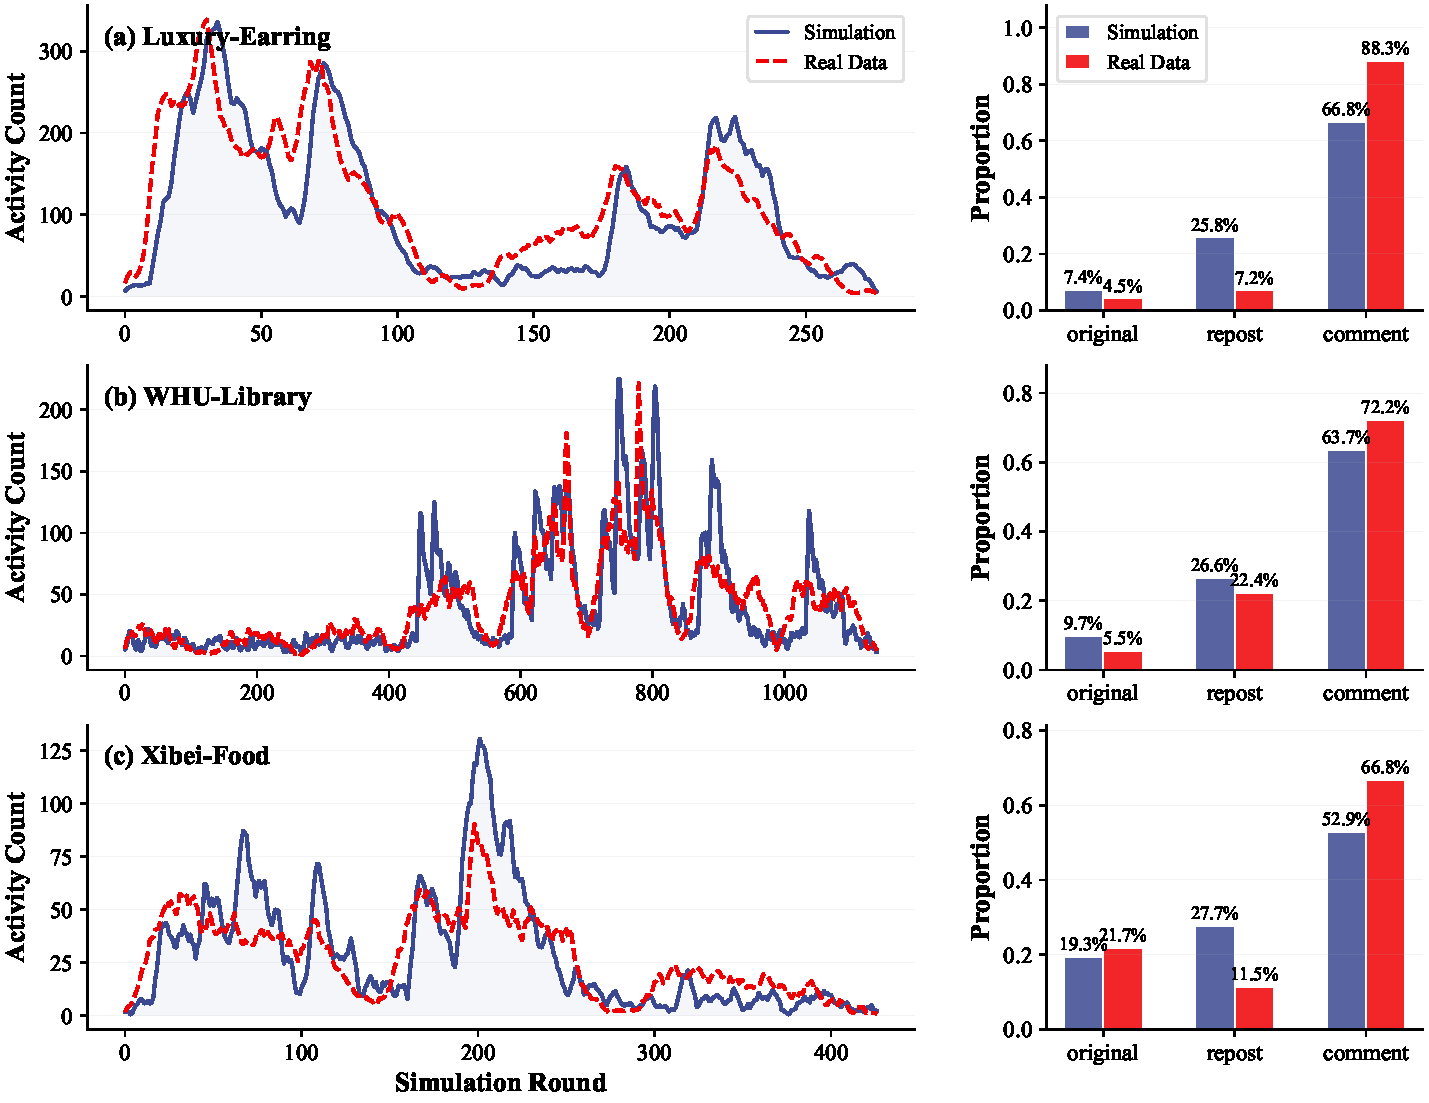
\includegraphics[width=0.75\textwidth]{fig_three_event_calibration.pdf}
\caption{三个事件的行为热度与分布校准结果。每行对应一个事件（(a)~天价耳环、(b)~武大图书馆、(c)~西贝预制菜），左侧为模拟与真实数据的活跃度时序对比，右侧为行为类型的比例分布对比。}
\label{fig:three_event_calibration}
\end{figure}

\end{document}

